%% (Master) Thesis template
% Template version used: v1.4
%
% Largely adapted from Adrian Nievergelt's template for the ADPS
% (lecture notes) project.


% We use the memoir class because it offers a many easy to use features.
\documentclass[11pt,a4paper,titlepage,oneside]{memoir}

\setlrmarginsandblock{3.2cm}{3.2cm}{*}

%% Packages
%% ========

%% LaTeX Font encoding -- DO NOT CHANGE
%\usepackage[OT1]{fontenc}

%% Babel provides support for languages.  'english' uses British
%% English hyphenation and text snippets like "Figure" and
%% "Theorem". Use the option 'ngerman' if your document is in German.
%% Use 'american' for American English.  Note that if you change this,
%% the next LaTeX run may show spurious errors.  Simply run it again.
%% If they persist, remove the .aux file and try again.
%\usepackage[english]{babel}

%% Input encoding 'utf8'. In some cases you might need 'utf8x' for
%% extra symbols. Not all editors, especially on Windows, are UTF-8
%% capable, so you may want to use 'latin1' instead.
%\usepackage[utf8]{inputenc}

%% This changes default fonts for both text and math mode to use Herman Zapfs
%% excellent Palatino font.  Do not change this.
%\usepackage[sc]{mathpazo}

%% The AMS-LaTeX extensions for mathematical typesetting.  Do not
%% remove.
\usepackage{amsmath,amssymb,amsfonts,amsthm}

%% NTheorem is a reimplementation of the AMS Theorem package. This
%% will allow us to typeset theorems like examples, proofs and
%% similar.  Do not remove.
%% NOTE: Must be loaded AFTER amsmath, or the \qed placement will
%% break
% \usepackage[amsmath,thmmarks]{ntheorem}

%% LaTeX' own graphics handling
% \usepackage{graphicx}


%% We unfortunately need this for the Rules chapter.  Remove it
%% afterwards; or at least NEVER use its underlining features.
%\usepackage{soul}

%% This allows you to add .pdf files. It is used to add the
%% declaration of originality.
\usepackage{pdfpages}

%% Some more packages that you may want to use.  Have a look at the
%% file, and consult the package docs for each.
%% See the TeXed file for more explanations

%% [OPT] Multi-rowed cells in tabulars
%\usepackage{multirow}

%% [REC] Intelligent cross reference package. This allows for nice
%% combined references that include the reference and a hint to where
%% to look for it.
%\usepackage{varioref}

%% [OPT] Easily changeable quotes with \enquote{Text}
%\usepackage[german=swiss]{csquotes}

%% [REC] Format dates and time depending on locale
%\usepackage{datetime}

%% [OPT] Provides a \cancel{} command to stroke through mathematics.
%\usepackage{cancel}

%% [NEED] This allows for additional typesetting tools in mathmode.
%% See its excellent documentation.
\usepackage{mathtools}

%% [ADV] Conditional commands
%\usepackage{ifthen}

%% [OPT] Manual large braces or other delimiters.
%\usepackage{bigdelim, bigstrut}

%% [REC] Alternate vector arrows. Use the command \vv{} to get scaled
%% vector arrows.
%\usepackage[h]{esvect}

%% [NEED] Some extensions to tabulars and array environments.
%\usepackage{array}

%% [OPT] Postscript support via pstricks graphics package. Very
%% diverse applications.
%\usepackage{pstricks,pst-all}

%% [?] This seems to allow us to define some additional counters.
%\usepackage{etex}

%% [ADV] XY-Pic to typeset some matrix-style graphics
%\usepackage[all]{xy}

%% [OPT] This is needed to generate an index at the end of the
%% document.
%\usepackage{makeidx}

%% [OPT] Fancy package for source code listings.  The template text
%% needs it for some LaTeX snippets; remove/adapt the \lstset when you
%% remove the template content.
%\usepackage{listings}
%\lstset{language=TeX,basicstyle={\normalfont\ttfamily}}

%% [REC] Fancy character protrusion.  Must be loaded after all fonts.
\usepackage{microtype}

%% [REC] Nicer tables.  Read the excellent documentation.
%\usepackage{booktabs}

%\usepackage[draft,bookmarks=true]{hyperref}

\usepackage[normalem]{ulem}
\usepackage{thmtools}
\usepackage[
  n,
  operators,
  advantage,
  sets,
  adversary,
  landau,
  probability,
  notions,
  logic,
  ff,
  mm,
  primitives,
  events,
  complexity,
  oracles,
  asymptotics,
  keys]{cryptocode}


%% Our layout configuration.  DO NOT CHANGE.
%% Memoir layout setup

%% NOTE: You are strongly advised not to change any of them unless you
%% know what you are doing.  These settings strongly interact in the
%% final look of the document.

% Dependencies
\usepackage{ETHlogo}

% Turn extra space before chapter headings off.
\setlength{\beforechapskip}{0pt}

\nonzeroparskip
\parindent=0pt
\defaultlists

% Chapter style redefinition
\makeatletter

\if@twoside
  \pagestyle{Ruled}
  \copypagestyle{chapter}{Ruled}
\else
  \pagestyle{ruled}
  \copypagestyle{chapter}{ruled}
\fi
\makeoddhead{chapter}{}{}{}
\makeevenhead{chapter}{}{}{}
\makeheadrule{chapter}{\textwidth}{0pt}
\copypagestyle{abstract}{empty}

\makechapterstyle{bianchimod}{%
  \chapterstyle{default}
  \renewcommand*{\chapnamefont}{\normalfont\Large\sffamily}
  \renewcommand*{\chapnumfont}{\normalfont\Large\sffamily}
  \renewcommand*{\printchaptername}{%
    \chapnamefont\centering\@chapapp}
  \renewcommand*{\printchapternum}{\chapnumfont {\thechapter}}
  \renewcommand*{\chaptitlefont}{\normalfont\huge\sffamily}
  \renewcommand*{\printchaptertitle}[1]{%
    \hrule\vskip\onelineskip \centering \chaptitlefont\textbf{\vphantom{gyM}##1}\par}
  \renewcommand*{\afterchaptertitle}{\vskip\onelineskip \hrule\vskip
    \afterchapskip}
  \renewcommand*{\printchapternonum}{%
    \vphantom{\chapnumfont {9}}\afterchapternum}}

% Use the newly defined style
\chapterstyle{bianchimod}

\setsecheadstyle{\Large\bfseries\sffamily}
\setsubsecheadstyle{\large\bfseries\sffamily}
\setsubsubsecheadstyle{\bfseries\sffamily}
\setparaheadstyle{\normalsize\bfseries\sffamily}
\setsubparaheadstyle{\normalsize\itshape\sffamily}
\setsubparaindent{0pt}

% Set captions to a more separated style for clearness
\captionnamefont{\bfseries\footnotesize}
\captiontitlefont{\footnotesize}
\setlength{\intextsep}{16pt}
\setlength{\belowcaptionskip}{1pt}

% Set section and TOC numbering depth to subsection
\setsecnumdepth{subsection}
\settocdepth{subsection}

%% Titlepage adjustments
\pretitle{\vspace{0pt plus 0.7fill}\begin{center}\HUGE\sffamily\bfseries}
\posttitle{\end{center}\par}
\preauthor{\par\begin{center}\let\and\\\Large\sffamily}
\postauthor{\end{center}}
\predate{\par\begin{center}\Large\sffamily}
\postdate{\end{center}}

\def\@advisors{}
\newcommand{\advisors}[1]{\def\@advisors{#1}}
\def\@department{}
\newcommand{\department}[1]{\def\@department{#1}}
\def\@thesistype{}
\newcommand{\thesistype}[1]{\def\@thesistype{#1}}

\renewcommand{\maketitlehooka}{\noindent\ETHlogo[2in]}

\renewcommand{\maketitlehookb}{\vspace{1in}%
  \par\begin{center}\Large\sffamily\@thesistype\end{center}}

\renewcommand{\maketitlehookd}{%
  \vfill\par
  \begin{flushright}
    \sffamily
    \@advisors\par
    \@department, ETH Z\"urich
  \end{flushright}
}

\checkandfixthelayout

\setlength{\droptitle}{-48pt}

\makeatother

% This defines how theorems should look. Best leave as is.
\theoremstyle{plain}
%\setlength\theorempostskipamount{0pt}

%%% Local Variables:
%%% mode: latex
%%% TeX-master: "thesis"
%%% End:


%% Theorem environments.  You will have to adapt this for a German
%% thesis.
%% Theorem-like environments

\numberwithin{equation}{chapter}

\declaretheorem[numberwithin=chapter,name=Theorem]{thm}
\declaretheorem[numberlike=thm,name=Conjecture]{conjecture}
\declaretheorem[numberlike=thm,name=Proposition]{prop}
\declaretheorem[numberlike=thm,name=Lemma]{lemma}
\declaretheorem[numberlike=thm,name=Corollary]{corollary}
\declaretheorem[numberlike=thm,name=Definition]{defn}

\newenvironment{sketch}{%
  \renewcommand{\proofname}{Proof Sketch}\proof}{\endproof}

%% Helpful macros.
%% Custom commands
%% ===============

%% Shortcuts
\newcommand{\deq}{\coloneqq\,}
\newcommand\m[1]{\begin{bmatrix}#1\end{bmatrix}} 
\newcommand\mdts[2]{\m{#1_1 \\ \vdots \\ #1_{#2}}}
\newcommand\mtdts[2]{\m{#1_1 & \cdots & #1_{#2}}^\top}
\newcommand\dts[2]{#1_1, \dots, #1_{#2}}

%% Cryptography stuff
\newcommand{\A}{\mathcal{A}}
\newcommand{\F}{\mathds{F}}
\newcommand{\K}{\mathcal{K}}
\newcommand{\X}{\mathcal{X}}
\newcommand{\BC}{\mathcal{E}}


%% Linicrypt stuff
\renewcommand{\v}{\boldsymbol}

\renewcommand{\P}{\mathcal{P}}
\renewcommand{\A}{\mathcal{A}}
\renewcommand{\PH}[1][]{\P^\H_{\mathsf{#1}}}
\newcommand{\PE}[1][]{\P^\BC_{\mathsf{#1}}}

\newcommand{\M}{\boldsymbol{M}}
\newcommand{\Inp}{\boldsymbol{I}}
\newcommand{\I}{\boldsymbol{I}}
\newcommand{\Out}{\boldsymbol{O}}
\renewcommand{\O}{\boldsymbol{O}}
\newcommand{\Q}{\boldsymbol{Q}}
\newcommand{\B}{\boldsymbol{B}}
\newcommand{\Id}{\mathds{1}}

\newcommand{\C}{\mathcal{C}}
\newcommand{\Fix}{\mathcal{F}}
\newcommand{\Cfix}{\C_\textrm{fixed}}
\newcommand{\Ccs}{\C_\textrm{cs}}

\renewcommand{\H}{H}
\newcommand{\E}{E}
\newcommand{\D}{D}

\newcommand{\For}{\mathsf{Forward}}
\newcommand{\Back}{\mathsf{Backward}}
\newcommand{\is}{{i^*}}

\newcommand{\vbase}{\v v_\base}
\renewcommand{\vk}{\v k}
\newcommand{\vx}{\v x}
\newcommand{\vy}{\v y}
\newcommand{\vq}{\v q}
\newcommand{\va}{\v a}
\newcommand{\vi}{\v i}
\newcommand{\vo}{\v o}
\newcommand{\ve}{\v e}
\newcommand{\vv}{\v v}

\newcommand{\out}{\mathsf{out}}
\newcommand{\inp}{\mathsf{in}}
\newcommand{\base}{\mathsf{base}}
\newcommand{\Base}{\F^\base}
\newcommand{\spn}{\mathsf{span}}
\newcommand{\rows}{\mathsf{rows}}
\newcommand{\sol}{\mathsf{sol}}

% cryptocode setup
\setlength\pcbodylinesep{-0.2\baselineskip}
\setlength\pcheadlinesep{0.1\baselineskip}
\createprocedureblock{pcbl}{boxed}{}{}{beginline=\t}
\createprocedureblock{pcb}{center,boxed}{}{}{beginline=\t}



\usepackage[backend=bibtex,style=alphabetic]{biblatex}
\addbibresource{refs.bib} 
\addbibresource{crypto.bib} 

%% Make document internal hyperlinks wherever possible. (TOC, references)
%% This MUST be loaded after varioref, which is loaded in 'extrapackages'
%% above.  We just load it last to be safe.
%\usepackage[linkcolor=black,colorlinks=true,citecolor=black,filecolor=black]{hyperref}


%% Document information
%% ====================

\title{Modeling the Ideal Cipher in Linicrypt}
\author{Frederik Semmel}
\thesistype{Master Thesis}
\advisors{Advisors: Fabio Banfi, Ueli Maurer}
\department{Institute of Theoretical Computer Science}
\date{\today}

\begin{document}

\frontmatter

%% Title page is autogenerated from document information above.  DO
%% NOT CHANGE.
\begin{titlingpage}
  \calccentering{\unitlength}
  \begin{adjustwidth*}{\unitlength-24pt}{-\unitlength-24pt}
    \maketitle
  \end{adjustwidth*}
\end{titlingpage}

%% The abstract of your thesis.  Edit the file as needed.
\begin{abstract}
Linicrypt is a mathematical framework introduced by Carmer and Rosulek (Crypto 2016).
It is used to prove cryptographic properties of programs that only make calls to a random oracle and perform linear operations in a field $\F$.
We introduce new abstractions which allow us to extend Linicrypt to work with ideal ciphers instead of random oracles.
In Linicrypt, the execution of a program is viewed as a vector in a finite-dimensional vector space over $\F$.
We describe the set of such vectors in an alternative way and use this formalism to characterize a weakness regarding collision resistance called a collision structure.
Because of the new level of abstraction,
this characterization is applicable simultaneously in the ideal cipher model and the random oracle model.
We show that one can transform a program with a collision structure into its own attack
by performing a basis change on an algebraic representation of itself and then reversing its input and output.
The characterization is sound and complete in the case of Linicrypt programs making only a single query.
We apply these concepts in deriving an attack taxonomy for the \MD construction obtained from the 64 compression functions
introduced by Preneel, Govaerts, and Vandewalle (Crypto 1993).
\end{abstract}


%% TOC with the proper setup, do not change.
\cleartorecto
\tableofcontents
\mainmatter

\chapter{Introduction}


\chapter{Preliminaries}

\section{Linicrypt}
\subsection{Definition of a Linicrypt program}

The Linicrypt model for cryptographic constructions was introduced by Carmer \& Rosulek in \cite{C:CarRos16}.
Summarizing the formalization from that paper,
a pure Linicrypt program $\P$ is a straight line program
whose intermediate variables are elements in a field $\F$.
% TODO maybe operation isn't right
The only operations allowed to create an intermediate variable are:
\begin{itemize}
  \item Retrieve an input, which is in $\F$
  \item Perform a linear combination of existing internal variables with fixed parameters
  \item Call a random oracle $\H: \{0,1\}^* \times \F^* \to \F$
  \item Sample from $\F$ uniformly
\end{itemize}
Finally, the program $\P$ is allowed to output one or more of its variables.

Below is an example of a Linicrypt program $\P^\H$,
% TODO Linicrypt is actually a tuple of CMD's ... should I specify that? Maybe in the 
% block cipher part.
written in conventional pseudocode on the left and in explicit Linicrypt on the right. 

\begin{pchstack}[center, space=0.4cm]
  \pcbl[valign=c]{$\P^\H(x, y)$}{
    r \sample \F \\
    \pcreturn \H(x+r) + y
  }
  \pseudocode[valign=c]{\rightsquigarrow}
  \pcbl[valign=c]{$\P^\H(x, y)$}{
    v_1 \deq x \\
    v_2 \deq y \\
    v_3 \sample \F \\
    v_4 \deq v_1 + v_3 \\
    v_5 \deq \H(v_4) \\
    v_6 \deq v_5 + v_2 \\
    \pcreturn (v_6)
  }
\end{pchstack}

We will usually work with programs in conventional pseudocode and use suggestive names for the intermediate variables instead of $v_i$.
Nevertheless, one should keep in mind,
that such programs could be formalized as a sequence of Linicrypt commands,
each generating a new intermediate variable.
The superscript $\H$ is used to highlight that $\P$ has access to a random oracle.
As this is often clear from the context, this superscript will usually be dropped.
When a Linicrypt program contains no sampling operations it is called a deterministic Linicrypt program. 
In the context of collision resistance this is the case we care about the most.

\subsection{Type of Adversaries}
The Linicrypt model only imposes computational restrictions on the cryptographic constructions,
not on the adversaries.
We consider computationally unbounded adversaries $\A$,
which have bounded access to the random oracle $\H$.
Therefore, the behavior of an adversary is described in terms of the number of queries it makes.
The additional power granted to an adversary by allowing unbounded computations is usually not helpful in this model.
For example, we will show in the collision resistance case:
A successful attack is either not possible for information-theoretical reasons,
or it can be carried out by another Linicrypt program.

\subsection{Algebraic Representation}

One of the advantages of restricting the computational model is that one can characterize
Linicrypt programs with an algebraic representation.
We will introduce the concept of the algebraic representation as it was developed in previous Linicrypt papers.
Some definitions, in particular the definition of an oracle constraint, will be generalized in the next chapters.
Let $\P$ be a Linicrypt program with intermediate variables $v_1, \dots, v_n$.
These are sorted in the order in which they are created in the program.

A \textbf{base variable} is an intermediate variable which was created by retrieving an input,
calling the random oracle $\H$ or sampling from $\F$.
These are special, because they are not intrinsically linearly dependent of other intermediate variables.
A \textbf{derived variable} is one which is created by performing a linear combination of existing intermediate variables.
Note, that derived variables can always be uniquely written as linear combinations of base variables.
Let $\base$ be the number of base variables,
and we name them $\dts b \base \subset \{\dts v n\}$
We fix the ordering of the base variables by their order in $v_1, \dots, v_n$
We denote by $\vbase \in \Base$ the column vector
consisting of the values that the base variables take in a specific execution of $\P$.
That is, the $i$th component of $\vbase$ is set to the value of $b_i$ in that execution.
One should think of $\vbase$ as a vector containing the whole state of the program execution.
An intermediate variable, base or derived,
can then be seen as a linear function going from the vector space $\Fsp$ to its concrete value in $\F$.

Let $v_i$ be an intermediate variable.
% TODO here we make the distinction betwenn variable, it's value on an execution, is this cleaner? 
We define the \textbf{associated row vector} $\v v_i$ to be the unique row vector in $\Frowsp$ representing this function.
That means, that for every execution of $\P$:
If base variables take the values $\vbase$,
the variable $v_i$ has the value $\vv_i \vbase$.
Here we use the ordinary matrix product.
For example for the $i$th base variable $b_i$ we have 
$\v b_i = \m{0 & \cdots & 1 & \cdots & 0}$
where the $1$ is in the $i$th position.
We follow the convention used in the previous papers about Linicrypt to write matrices and vectors using a bold font.

The outputs of $\P$ can be described by a matrix with entries in $\F$.
Let $o_1, \dots, o_l \in \{v_1, \dots, v_n \}$ be the output variables of $\P$.
Then the \textbf{output matrix} $\O$ of $\P$ is defined by
\[
  \O =
  \begin{bmatrix}
  \v o_1\\
  \vdots \\
  \v o_l
  \end{bmatrix}.
\]
By the definition of the associated vectors $\v o_i$ we have
$
\O \vbase = 
  \begin{bmatrix} o_1 & \cdots & o_k \end{bmatrix}^\top
$.
The output matrix describes the linear correlations in the output of $\P$.

In the same way we also define the \textbf{input matrix} of $\P$.
If $i_1, \dots, i_k \in \{v_1, \dots, v_n\}$ are the intermediate variables created by retrieving an input,
then we write
\[
  \Inp = \begin{bmatrix}
  \v i_1 \\
  \vdots \\
  \v i_k
  \end{bmatrix}.
\]
As $i_1, \dots, i_k$ are base variables,
the rows of $\Inp$ are canonical basis row vectors.
If the Linicrypt program is written such that it first retrieves all its inputs,
then $\vi_m$ is simply the $m$'th canonical basis row vector. 

The input and output matrix describe the linear correlations between input and output of the program with respect to its base variables.
But the base variables are not completely independent of each other.
In fact, the relationship between the queries and answers to the random oracle $\H$ needs to be captured algebraically.
Let $a_i = H(t_i, (q_1, \dots, q_n))$ be an operation in $\P$.
The \textbf{associated oracle constraint} $c$ of this operation is the tuple
\[
  c = \left( t_i, \begin{bmatrix}
  \v q_1 \\
  \vdots \\
  \v q_n
  \end{bmatrix},
  \va_i \right)
	=
	(t_i, \Q_i, \va_i)
	.
\]
This should be interpreted as a constraint on $\vbase$, which requires
$\va_i \vbase = \H( t_i, \Q_i \vbase)$.
We denote the set of all (associated) oracle constraints of $\P$ by $\C$.

As we want the base variables to be linearly independent of each other,
we restrict ourselves to Linicrypt programs which don't make multiple calls to the random oracle with the same input.
In the language of the algebraic representation:
We assume wlog that no two constraints in $\C$ share the same $t$ and $\Q)$.

Wrapping up these definitions,
we define the \textbf{algebraic representation} of the program $\P$ to be the tuple $(\Inp, \O, \C)$.
A natural question that arises at this point is:
Does the algebraic representation determine the behavior of $\P$ completely?

The answer is yes, because the algebraic representation does not lose any relevant information about the operations executed in $\P$.
Informally, this is because the constraints in $\C$ have a particular form, which makes it clear in which order the oracles calls have to be executed.
Given the order, and using the input matrix, one can determine which variables used in the calls are retrieved from the input and which have to be sampled.
Finally, the output matrix completely describes how to construct the output from the input,
the results of the queries and the additional randomly sampled values. 

The authors of the original paper on Linicrypt \cite{C:CarRos16} establish a much stronger result for inputless programs.
First they define the normalized form of an algebraic representation.
It can be efficiently generated from any inputless program description.
They prove that two programs are indistinguishable if and only if their normalized algebraic representations are the same up to a basis change.
The concept of basis change will be discussed extensively in the next chapters.

\subsection{Characterizing Collision Resistance in Linicrypt}

In a paper by I. McQuoid, T. Swope and M. Rosulek
\cite[Characterizing Collision and Second-Preimage Resistance in Linicrypt]{TCC:McQSwoRos19},
the authors introduced a necessary condition for collision resistance
and second-preimage resistance for a deterministic Linicrypt program.

They identified two reasons why a \textit{deterministic} Linicrypt $\P$ program can fail to be second-preimage resistant.
One can describe them roughly as follows:
\begin{enumerate}
  \item It is degenerate, meaning that it doesn't use all of its inputs independently
  \item It has a collision structure,
    which means that one can change some intermediate variable and compute what the input needs to be to counteract this change
\end{enumerate}

Below are two example Linicrypt programs, $\P^\H_\textrm{deg}$ is degenerate and $\P^\H_\textrm{cs}$ has a collision structure.
\begin{pchstack}[center,space=2cm]
  \pcbl[valign=c]{$\P^\H_{\textrm{deg}}(x, y)$}{
    v \deq x + y \\
    \pcreturn H(v)
  }
  \pcbl[valign=c]{$\P^\H_{\textrm{cs}}(x, y)$}{
    w \deq x+y \\
    \pcreturn \H(w) + x
  }
\end{pchstack}
Note, that you can set $w' \neq w$ to any value,
then find an $x'$ such that the output of $\P^\H_{\textrm{cs}}$ stays the same,
and finally solve for $y'$ according to $w' = x' + y'$.

The authors show that for any deterministic Linicrypt program which is degenerate
or has a collision structure
second-preimage resistance (and hence also collision resistance) is completely broken.
The main result of \cite{C:CarRos16} is that they show that the converse of this is also true,
but only for Linicrypt programs which use distinct nonces in each call to the random oracle.
That is, if a such a Linicrypt program is not collision resistant,
then it either has a collision structure, or it is degenerate.
Furthermore, checking for degeneracy and existence of a collision structure can be done efficiently.

In the following chapters a similar result will be presented for a variant of Linicrypt
where we replace the random oracle $\H$ with an ideal cipher $\BC=(\E, \D)$.
Along the way,
we will merge the concepts of degeneracy and collision structure by considering degeneracy as an edge case of a collision structure.

\subsection{Notation}
We have already introduced some notational conventions.
For reference, we summarize the notation we are going throughout the argument.
Variables of a Linicrypt program and their values will be denoted with letters from the Latin alphabet in a regular font.
For example, depending on the context $x$ denotes a variable, or it denotes a concrete value in $\F$ a variable called $x$ takes in a specific execution of the program.
Their associated row vectors will have the same letter but in bold font, e.g. $\vx \in \Frowsp$.
Column vectors and matrices are also denoted by bold letters.
We use $\vbase \in \Fsp$ or $\vv \in \Fsp$ to denote the column vector containing all the values for the base variables in a program execution.
In a slight overload of notation,
we will denote both the canonical basis column vectors and the canonical basis row vectors by $\ve_i$.

Linicrypt statements are often about the span of the rows of matrices.
If $\v A \in \F^{a\times\base}$ for arbitrary $a \in \NN$,
then we define the rowspace of $\v A$ as $\rowsp(\v A) \coloneqq \spn(\rows(\v A)) \subseteq \Frowsp$.
Here we see $\rows$ as a function mapping a matrix in $\F^{a\times\base}$ the set of its rows, where each row is in $\Frowsp$.
Note that $\rowsp$ is sometimes defined as a subset of $\Fsp$ instead of $\Frowsp$.
We do not do this to simplify the notation in many statements,
and to emphasize that elements in $\rowsp(\v A)$ should be considered as possible intermediate variables.
For convenience, we also define for $\dts{\v A}{n}$ matrices with $\base$ columns: $\rowsp(\dts{\v A}{n}) \coloneqq \sum_i^n \rowsp(\v A_i)$.
The concept of rowspace is useful for example in the following style of arguments:
If $\v A\vv$ has been determined, then $\vw\vv$ is determined for any $\vw \in \rowsp(\v A)$.

The kernel of a matrix $\v A$ as above is also used in Linicrypt proofs.
As a reminder, $\ker(\v A) \coloneqq \{ \vv \in \Fsp\ \mid \v A \vv = 0\}$.
We will use the following facts from Linear Algebra:
\begin{align*}
  \rowsp(\v A)^\top &= \ker(\v A)^\perp \\
  (V_1 + V_2)^\perp &= V_1^\perp \cap V_2^\perp \quad \textrm{for $V_1$ and $V_2$ subspaces of $\Fsp$}
\end{align*}
For example:
If $\rowsp(\v A) + \rowsp(\v B) = \Frowsp$,
then $\v A \vv = \v A \vv'$ and $\v B \vv = \v B \vv'$ implies $\vv = \vv'$ for any $\vv, \vv' \in \Fsp$.

\subsection{Security Definitions}
We will use the following security definitions.
We only state them for ideal cipher model,
as that is the one we actually need in the argument.
Let $\P$ be a Linicrypt program taking $k$ inputs.
The collision game and the second-preimage game in the ideal cipher model are defined as:
\begin{pchstack}[center, space=0.4cm]
  \pcbl[]{$\crgame(\P, \A)$}{
  \textrm{instantiate an ideal cipher } \BC = (\E, \D) \\
  (\vi, \vi') \sample \A^\BC \\
  \pcreturn (\vi \neq \vi') \land \big(\P^\BC(\vi) = \P^\BC(\vi) \big)
  }
  \pcbl[]{$\sprgame(\P, \A)$}{
  \textrm{instantiate an ideal cipher } \BC = (\E, \D) \\
  \vi \sample \F^k \\
  \vi' \sample \A^\BC(\vi) \\
  \pcreturn (\vi \neq \vi') \land \big(\P^\BC(\vi) = \P^\BC(\vi) \big)
  }
\end{pchstack}

\begin{defn}[Collision Resistance]
  Let $\A$ be an adversary and $\P$ be a Linicrypt program.
  We define $\A$'s advantage as 
  \[
    \cradv[\A, \P] = \prob{\crgame(\P, \A) = 1}.
  \]
  We call $\P$ collision resistant if
  $\cradv[\A, \P]$ is negligible for all (possibly not efficient) adversaries $\A$.
\end{defn}

\begin{defn}[Second-preimage Resistance]
  Let $\A$ be an adversary and $\P$ be a Linicrypt program.
  We define $\A$'s advantage as 
  \[
    \spradv[\A, \P] = \prob{\sprgame(\P, \A) = 1}.
  \]
  We call $\P$ second-preimage resistant
  if $\spradv[\A, \P]$ is negligible for all (possibly not efficient) adversaries $\A$.
\end{defn}

These definitions are dependent on the choice of the field $\F$.
A result that limits the advantage of an adversary against a program usually depends on the size of the field $\F$.
If one wants to have security definitions depending on a security parameter $\lambda \in \NN$,
then one can choose a family of fields $\F_\lambda$ where $|\F_\lambda|$ is exponential in $\lambda$.
One can then only talk about the security of a family of programs $\P_\lambda$.
If the coefficients are in a subfield of every $\F_\lambda$,
e.g. $\{0,1\}$ as they are for most constructions,
then changing $\lambda$ will usually not affect the relevant properties of the program.
For example, if such a $\P_\lambda$ has a collision structure for some $\lambda$,
then it has a collision structure for all $\lambda$.

\chapter{Linicrypt with Ideal Ciphers}

\section{Revisiting Algebraic Representations}
We have defined the algebraic representation for any Linicrypt program.
A question that arises is: Which combination of matrices of the structure $(\M, \C)$
correspond to a Linicrypt program?
To answer this question, we need to define the terminology more carefully.

\begin{defn}
A random oracle constraint of dimension $\base$ with $k$ inputs is a tuple $(t, \v Q, \v a)$ for
$t \in \bin^*$, $\Q \in \F^{k \times \base}$ and $\va \in \F^{1 \times \base}$.
\end{defn}

We call $t$ the nonce and refer to $\Q$ and $\va$ as the query and answer to the random oracle.
Usually we just say constraint when the other variables are clear from the context.
The constraints $(t, \Q, \va)$ encodes a relationship between the base variables $\vbase \in \Base$ of a program.
Namely $\H(t, \Q \vbase) = \va \vbase$.
Because $\H$ is a well-defined function,
and not just any relation,
these requirements extend to the constraints.

\begin{defn}
A set of (random oracle) constraints $\C$ is well-defined if for any pair of constraints 
$c_i, c_j \in \C$ we have $(t_i,\Q_i) = (t_j, \Q_j) \implies \va_i = \va_j$.
\end{defn}

When we use a set of constraints, we will implicitly also require that it is well-defined.
Now we can characterize which sets of constraints correspond to a Linicrypt program.

\begin{defn}[Solvable]
Let $\C$ be a finite set of valid constraints.
$\C$ is (deterministically) solvable if there exists an ordering $(c_1, \dots, c_n)$ of $\C$
and a subspace $\Fix$ of $\Base$
such that for all $i=1, \dots n$:
\begin{enumerate}
\item
    $\spn(\Q_i) \subset \Fix + \spn \big(c_1, \dots, c_{i-1} \big)$
\item
    $\va_i \notin \Fix + \spn \big(c_1, \dots, c_{i-1} \big) + \spn(\Q_i)$
\item
    TODO or this notation
\item
    $\rows(\Q_i) \subset \spn \big(\Fix \cup \rows(c_1) \cup \dots \cup \rows(c_{i-1})\big)$
\item
    $\va_i \notin \spn \big(\Fix \cup \rows(c_1) \cup \dots \cup \rows(c_{i-1}) \cup \rows(\Q_i) \big)$
\end{enumerate}

We call $\Fix$ the solvable space (TODO or free space or fixable space or fixed space) of $\C$
and write $\sol(\C) = \Fix$.
We call $(c_1, \dots, c_n)$ the (solution) ordering of $\C$.
\end{defn}

If we construct the algebraic representation of a Linicrypt program $\P$,
we get a solvable set of constraints.
Indeed, the ordering of the constraints in the definition can be exactly the order of the corresponding queries in the execution of $\P$.
In this case, the solvable space would be the space spanned by the corresponding vectors to the input variables and the randomly sampled variables.

The other direction is also true.

\begin{lemma}[Solvable constraints]
    Let $\C$ be a set of solvable constraints and $k = \dim (\sol (\C))$.
    Let $\out \in \NN$ be arbitrary and $\inp \leq k$.
    Let $\M \in \F^{\out \times \base}$ be an arbitrary output matrix.
    Then there is a basis change $\B \in \F^{\base \times \base}$
    and a Linicrypt program $\P$ taking $\inp$ inputs
    such that $(\M, \C \B^{-1})$ is it's algebraic representation.
\end{lemma}

\begin{proof}
Let $(\vx_1, \dots, \vx_k)$ be a basis for $\sol(\C)$ and let $(c_1, \dots, c_n)$ be the ordering.
The new basis for $\Base$ is $(\vx_1, \dots, \vx_k, \va_1, \dots, \va_n)$.
\[
    \B = 
    \begin{bmatrix}
\vx_1 &
\dots &
\vx_k &
\va_1 &
\dots &
\va_n
    \end{bmatrix}^\top
\]
TODO or
\[
    \B =
    \begin{bmatrix}
\vx_1 \\
\vdots \\
\vx_k \\
\va_1 \\
\vdots \\
\va_n
    \end{bmatrix}
\]

Then we define the constraints $\C'$ via $t_i' = t_i$, $\Q_i' B = \Q_i$ and $\va_i' B = \va_i$.
Note, that, as $\C$ is solvable via the ordering $(c_1, \dots, c_n)$,
these constraints have the form
\begin{align*}
\Q_i' &= \begin{bmatrix} \lambda^i_1 & \cdots & \lambda^i_{i-1} & 0 & 0 & \cdots & 0 \end{bmatrix} \qquad \textrm{for} \quad \lambda^i_j \in \F \\
\va_i' &= \begin{bmatrix} \;0\;\, & \dots & \;\;\;0\;\;\; & 1 & 0 & \dots & 0 \end{bmatrix}
\end{align*}

This is the correct form for an algebraic representation of a program $\P$ taking $\inp \leq k$ inputs,
randomly sampling the next $k - \inp \geq 0$ base variables,
and outputting according to $\M$.
\end{proof}

TODO maybe switch to using input matrices, this would maybe clean things up later
\begin{lemma}[Solvable constraints]
Let $\C$ be a set of solvable constraints and $k = \dim (\sol (\C))$.
Let $\out \in \NN$ be arbitrary and $\inp \leq k$.
Let $\M \in \F^{\out \times \base}$ be arbitrary and $\Inp \in \F^{\inp \times \base}$ such that $\spn(\Inp) \subseteq \sol(\C)$.
Then there is a basis change $\B \in \F^{\base \times \base}$ and a Linicrypt program $\P$
such that $(\Inp \B^{-1}, \M\B^{-1}, \C \B^{-1})$ is it's algebraic representation.
\end{lemma}

\section{Revisiting Collision Structures}
Using this language we can argue about the invertibility of a Linicrypt program and about the possibility to directly calculate second preimages.
Let $\P = (\M, \C)$ be a Linicrypt program.

\begin{lemma}
    $\P$ is invertible if $\rows(\M) \subseteq \sol(\C).$
\end{lemma}

\begin{proof}
TODO
\end{proof}

\begin{lemma}
    $\P$ has a collision structure
    if $\C = \C_{\textrm{fixed}} \sqcup \C_{\textrm{cs}}$ such that
    \begin{equation}
        \sol(\C_\textrm{cs}) \supset \spn\big(\rows(\C_\textrm{fixed}) \cup \rows(\M)\big).
    \end{equation}
\end{lemma}
\begin{proof}
TODO
\end{proof}

Note, that it is crucial that the space on the left is $\supset$ and not only $\supseteq$,
as this gives the extra degree of freedom to find a different preimage.
This is the same role that $w'$ plays in the example from \cite{RMS20}.

This characterization directly includes the case of degeneracy,
because then $\Ccs = \{\}$ and $\sol(\Ccs) = \Base$,
while degeneracy means precisely $\Base \supset \spn(\rows(\C) \cup \rows(\M))$.

The following example was slightly adapted so that it is invertible.

\pcb[valign=c]{$\PE[inv,1](x,y,z)$}{
    w = \H(x) + \H(z) + y \\
    \pcreturn (\H(w) + x, z)
}

\begin{align*}
\M    &= \begin{vmatrix}
            1 & 0 & 0 & 0 & 0 & 1 \\
            0 & 0 & 1 & 0 & 0 & 0 
            \end{vmatrix} \\
\vq_1 &= \begin{vmatrix}1 & 0 & 0 & 0 & 0 & 0\end{vmatrix} \\
\va_1 &= \begin{vmatrix}0 & 0 & 0 & 1 & 0 & 0\end{vmatrix} \\
\vq_2 &= \begin{vmatrix}0 & 0 & 1 & 0 & 0 & 0\end{vmatrix} \\
\va_2 &= \begin{vmatrix}0 & 0 & 0 & 0 & 1 & 0\end{vmatrix} \\
\vq_3 &= \begin{vmatrix}0 & 1 & 0 & 1 & 1 & 0\end{vmatrix} \\
\va_3 &= \begin{vmatrix}0 & 0 & 0 & 0 & 0 & 1\end{vmatrix} \\
\end{align*}

Note, that $(c_3, c_2, c_1)$ is an ordering solving $\C$ and $\rows(M) \subset \sol(\C)$.

TODO finish typing this example

\section{Adapting the Linicrypt model to use block ciphers}

In this chapter we modify the Linicrypt model to make use of the ideal cipher model instead of the random oracle model.
This means that a Linicrypt program gets access to a block cipher $\mathcal{E} = (E, D)$ where $E$ and $D$ are functions $\F \times \F \to \F$
instead of the hash function $\H : \{0,1\}^* \times \F^* \to \F$.
By the definition of a block cipher,
$\E_k := \E(k, \cdot)$ is a permutation of $\F$ for all $k \in \F$ and
$\D_k := \D(k, \cdot)$ is its inverse.
In the ideal cipher model, we assume that the block cipher has no weakness.
This is modeled by choosing each permutation $\E_k$ uniformly at random at the beginning of every security game.

The command $y = \E(k, x)$ in a Linicrypt program has to be treated differently from the command $y = \H(k, x)$ when considering collision resistance,
because an attacker has access to the deterministic Linicrypt program and both directions of the block cipher $\mathcal{E} = (\E, \D)$.
Consider these two programs, $\PH$ in standard Linicrypt and $\PE$ in ideal cipher Linicrypt.

\begin{pchstack}[center,space=2cm]
  \pcbl[valign=c]{$\PH(k, x)$}{
    \pcreturn \H(k,x)
  }
  \pcbl[valign=c]{$\PE(k, x)$}{
    \pcreturn \E(k,x)
  }
\end{pchstack}
While $\PH$ is collision resistant, it is trivial to find second preimages for $\PE$
For any $k' \in \F$ the pair $(k', \D(k', \E(k, x)))$ is a second preimage to $(k,x)$.

This invertibility property of block ciphers has to be taken into account
in both the algebraic representation and the characterization of collision resistance.

\subsection{Algebraic representation for ideal cipher Linicrypt}

Let $\P$ be a ideal cipher Linicrypt program. For each query to $\E$ of the form $y =
\E(k,x)$ we define the \textbf{associated ideal cipher constraint} $(\E, \v k, \v x, \v y)$.
Each query to $\D$ of the form $x = \D(k, y)$, is
associated with the constraint $(\D, \v k, \v y, \v x)$.

As with standard Linicrypt,
we want to exclude programs that make unnecessary queries to the block cipher.
This way the base variables are linearly independent,
except for the dependencies the adversary might introduce by carefully choosing the input.
Hence we assume wlog that no two constraints have the same $(\E, \v k, \v x)$ or $(\D, \v k, \v y)$.

With ideal ciphers there is a second way to make an unnecessary query.
That is by first computing $y = \E(k,x)$ and then $x' = \D(k, y)$.
As $\D_k$ is the inverse of $\E_k$ we have $x = x'$ although $\v x$ and $\v x'$ are linearly independent.


Therefore for all $\v k, \v x, \v x', \v y, \v y' \in \Base$ we can assume there are no two constraints
$(\E, \v k,\v x, \v y)$ and $(\D, \v k, \v y, \v x')$ in $\C$ for $\v x \neq \v x'$.
Neither can there be $(\D, \v k,\v y, \v x)$ and $(\E, \v k, \v x, \v y')$ in $\C$ for $\v y \neq \v y'$.

TODO: Maybe it is simpler with equivalence relation called always colliding queries
\begin{align*}
    (\E, \v k,\v x, \v y) &\sim (\E, \v k, \v x, \v y') \\ 
    (\E, \v k,\v x, \v y) &\sim (\D, \v k, \v y, \v x') \\
    (\D, \v k,\v y, \v x) &\sim (\D, \v k, \v y, \v x') \\
    (\D, \v k,\v y, \v x) &\sim (\E, \v k, \v x, \v y')
\end{align*}
And saying that no two constraints in $\C$ are in the same equivalence class.
This might be cleaner, if the equivalence relation used later to analyze repeated nonces case is defined similarly.

\section{Collision Structure}

To explain the concept of a collision structure, we will make use of an example.
Consider the following Linicrypt program:
\pcb[valign=c]{$\PE[col,1](a,b,c)$}{
    w = E(c, b+c) + a \\
    \pcreturn c + \E(w,b)
}
A second preimage to $(a,b,c)$ can be found by the following procedure:
Choose some $w' \neq w$.
It will turn out, that even choosing $w'$ at random,
one can calculate what the other base variables need to be such that the output stays the same.
As we want $c + \E(w,b) = c' + \E(w', b')$ we can again choose any $b'$ and compute $c'$. 
Finally, we can compute $a'$ from the equation $w' = \E(c', c' + b') + a'$

One can more easily see that such a procedure is possible by looking at the algebraic representation of $\PE[col,1]$.
In order to highlight which are the base variables, we rewrite the program a bit more explicitly.
\pcb[valign=c]{$\PE[col,1](a,b,c)$}{
    k_1 = c \\
    x_1 = b+c \\
    y_1 = \E(k_1, x_1) \\
    k_2 = y_1 + a \\
    x_2 = b \\
    y_2 = \E(k_2, x_2) \\
    \pcreturn c + y_2
}
The base variables are $(a, b, c, y_1, y_2)$ and the algebraic representation is
\[
    \M = \begin{bmatrix} 0, 0, 1, 0, 1 \end{bmatrix} 
        \qquad \C = \{(\E, \v k_1, \v x_1, \v y_1), (\E, \v k_2, \v x_2, \v y_2)\}
\]
where
\begin{align*}
\v k_1 &= \begin{bmatrix} 0, 0, 1, 0, 0 \end{bmatrix} \\
\v x_1 &= \begin{bmatrix} 0, 1, 1, 0, 0 \end{bmatrix} \\
\v y_1 &= \begin{bmatrix} 0, 0, 0, 1, 0 \end{bmatrix} \\
\v k_2 &= \begin{bmatrix} 1, 0, 0, 1, 0 \end{bmatrix} \\
\v x_2 &= \begin{bmatrix} 0, 1, 0, 0, 0 \end{bmatrix} \\
\v y_2 &= \begin{bmatrix} 0, 0, 0, 0, 1 \end{bmatrix}.
\end{align*}

We can formulate the previous attack from in terms of the algebraic representation.
The task is to find a $\v v_\base' = [a', b', c', y_1', y_2'] \neq \v v_\base$ such that:
\begin{align}
\label{constraint_output}
\PE[col,1](a', b', c') = \M \vbase' &= \M \vbase = \PE[col,1](a,b,c) \\
\label{constraint_cipher_1}
y_1' = \vy_i \vbase' &=  \E(\vk_1 \vbase'\,, \; \vx_1 \vbase')\\
\label{constraint_cipher_2}
y_2' = \vy_i \vbase' &=  \E(\vk_2 \vbase'\,, \; \vx_2 \vbase')
\end{align}

We can fulfill these requirements step by step.
First, we constrain $\vbase'$ by requiring 
\[
    \M \vbase' = \M \vbase.
\]
This reduces the dimension of the space of possible solutions for $\vbase'$ to 4,
as $\M \vbase$ is in the range of $\M$ by definition.
Now note, that neither $\vk_2$ nor $\vx_2$ are in the span of $\rows(\M)$.
Therefore we can choose $k_2'$ and $x_2'$ at random such that $(k_2', x_2') \neq (k_2, x_2)$,
and constrain $\vbase'$ by requiring
\[
    \vk_2 \vbase' = k_2' \quad \textrm{and} \quad \vx_2 \vbase' = x_2'.
\]
Now we can compute $y_2' = \E(k_2', x_2')$ and add constraint \eqref{constraint_cipher_2}.
This constraint is compatible with the previous constraints because $\vy_2$ is not in the span of
$\rows(\M) \cup \{\vk_2, \vx_2\}$.
The dimension of the subspace of solutions is now 1, as we have added 4 one-dimensional constraints.

Now one only needs to fulfill constraint \eqref{constraint_cipher_1}.
As $\vk_1$ and $\vx_1$ are in the span of
$\rows(\M) \cup \{\vk_2, \vx_2, \vy_2\}$ the intermediate variables $k_1'$ and $x_1'$ are uniquely determined.
E.g. $\vk_1 = \M - \vy_2$ and therefore $k_1' = \PE[col,1](a,b,c) - y_2'$.

Finally, note that 
$\vy_1 \notin \spn\big( \rows(\M) \cup \{ \vk_2, \vx_2, \vy_2 \} \cup \{ \vk_1, \vx_1 \} \big)$.
Therefore, adding the constraint
\[
    \vy_1 \vbase' = y_1' = \E(k_1', x_1')
\]
reduces the solution space of possible $\vbase'$ to a single point in $\Base$.
We know that $\vbase' \neq \vbase$ because $(k_2, x_2') \neq (k_2, x_2)$.
The only way to produce different intermediate variables in a deterministic program is to choose different input,
hence $(a',b',c') \neq (a,b,c)$.

This example would have worked exactly the same if we replaced $\E$ with $\H$.
What follows is an example where the invertibility property of $\E_k$ plays a role.

\begin{pchstack}[center, space=2cm]
    \pcbl[valign=c]{$\PE[col,2](a,b,c)$}{
        k_1 = c \\
        x_1 = b \\
        y_1 = \E(k_1, x_1) \\
        k_2 = a \\
        x_2 = y_1 \\
        y_2 = \E(k_2, x_2) \\
        \pcreturn y_1 + y_2
    }
    \pseudocode[valign=c]{
        \M    = \begin{bmatrix}0,0,0,1,1\end{bmatrix} \\
        \vk_1 = \begin{bmatrix}0,0,1,0,0\end{bmatrix} \\
        \vx_1 = \begin{bmatrix}0,1,0,0,0\end{bmatrix} \\
        \vy_1 = \begin{bmatrix}0,0,0,1,0\end{bmatrix} \\
        \vk_2 = \begin{bmatrix}1,0,0,0,0\end{bmatrix} \\
        \vx_2 = \begin{bmatrix}0,0,0,1,0\end{bmatrix} \\
        \vy_2 = \begin{bmatrix}0,0,0,0,1\end{bmatrix} 
    }
\end{pchstack}
For this program there is a similar procedure to find second preimages.
As before, the first constraint is $\M $
In this case we can fix $\vk_2 \vbase' = k_2' = k_2$, $\vx_2 \vbase' = x_2' = x_2$ and $\vy_2 \vbase' = y_2' = y_2$.
Therefore condition \eqref{constraint_cipher_2} is fulfilled trivially.
After adding these 4 constraints the solutions space is still 1-dimensional.
Note, that $\vy_1 = \vx_2$ and it is therefore already fixed at this point,
hence to fulfill \eqref{constraint_cipher_1} we have to make use of the invertibility property of $\E_k$.
Because
\begin{align*}
    \vy_1 \vbase' &= \E(\vk_1 \vbase', \vx_1 \vbase') \\
    \iff \vx_1 \vbase' &= \D(\vk_1 \vbase', \vy_1 \vbase'),
\end{align*}
we can choose a random $k_1' \neq k_1$ and compute $x_1' = \D(k_1', y_1')$ in order to fulfill (3.1).
With this fifth constraint we have found a single $\vbase' \neq \vbase$.

We want to briefly summarize the conditions for this kind of second preimage attack.
Let $\P'$ denote the execution of 
\begin{itemize}
\item
    Some ideal cipher constraints are fulfilled by setting the intermediate variables in $\P(a',b',c')$ to the same value as in $\P(a,b,c)$ 
\item
    There is some constraint for which either the input or the output is undetermined by the previously fixed intermediate variables
\item
    For this constraint and all following constraint one can iteratively call the ideal cipher $\BC$ to set the intermediate variables such that the constraints are fulfilled.
    This is only possible, if the either the output or the input is undetermined by previously fixed variables.
\end{itemize}


\begin{defn}[Collision structure]
Let $\P = (\M, \C)$ be a Linicrypt program with $|\C| = n$.
A \textbf{collision structure} for $\P$ is an index $1 \leq i^* \leq n$, an ordering $(c_1, \dots, c_n)$ of $\C$ for $c_i = (Op_i, \v k_i, \v q_i,\v a_i)$
and a tuple $(dir_{i^*}, \dots, dir_n)$ for $dir_i \in \{\For, \Back\}$,
such that the following two conditions hold:
\begin{enumerate}
\item 
Let $\mathcal{F}_\is = \{
    \v k_1, \dots, \v k_{i^* -1},
    \v q_1, \dots, \v q_{i^* -1},
    \v a_1, \dots, \v a_{i^* -1}
    \}$. One of the following is true:
        \begin{enumerate}
    \item $dir_\is = \For \quad$ and 
        $\quad
            \spn\big(\{ \v k_{i^*}, \v q_{i^*} \}\big) \nsubseteq
            \spn\big( \mathcal{F}_\is \cup \rows\left(\M\right) \big)
        $
    \item $dir_\is = \Back \quad$ and 
        $\quad
            \spn\big(\{ \v k_{i^*}, \v a_{i^*} \}\big) \nsubseteq
            \spn\big( \mathcal{F}_\is \cup \rows\left(\M\right) \big)
        $
\end{enumerate}
\item For all $j \geq i^*$ let $\mathcal{F}_j = \{
    \v k_1, \dots, \v k_{j -1},
    \v q_1, \dots, \v q_{j -1},
    \v a_1, \dots, \v a_{j -1}
    \}$. One of the following is true:
\begin{enumerate}
    \item $dir_j = \For \quad$ and 
        $\quad
        \v a_j \notin \spn\big(
        \mathcal{F}_j
        \cup \{ \v k_j, \v q_j\}
        \cup \rows\left(\M\right)
        \big)
        $
    \item $dir_j = \Back \quad$ and 
        $\quad
        \v q_j \notin \spn\big(
        \mathcal{F}_j
        \cup \{ \v k_j, \v a_j\}
        \cup \rows\left(\M\right)
        \big)
        $
\end{enumerate}
\end{enumerate}
\end{defn}

TODO: Remove this wordy definition.
All the info from here should be integrated into the example

\begin{defn}[Collision structure]
Let $\P = (\M, \C)$ be a Linicrypt program with $|\C| = n$.
A \textbf{collision structure} for $\P$ is an index $1 \leq i^* \leq n$, an ordering $(c_1, \dots, c_n)$ of $\C$ for $c_i = (Op_i, \v k_i, \v q_i,\v a_i)$
and a tuple $(dir_{i^*}, \dots, dir_n)$ for $dir_i \in \{\For, \Back\}$,
such that:
\begin{enumerate}
\item The $i^*$'th constraint is unconstrained by the output of $\P$ and previous fixed constraints.
Let $\mathcal{F} = \{
    \v k_1, \dots, \v k_{i^* -1},
    \v q_1, \dots, \v q_{i^* -1},
    \v a_1, \dots, \v a_{i^* -1}
    \}$
denote the vectors fixed by previous constraints in the ordering.
\begin{enumerate}
    \item if $dir_\is = \For$, the input of the query associated to $c_\is$ is unconstrained:
        \[
            \spn\big(\{ \v k_{i^*}, \v q_{i^*} \}\big) \nsubseteq
            \spn\big( \mathcal{F} \cup \rows\left(\M\right) \big)
        \]
    \item if $dir_\is = \Back$, the output of the query associated to $c_\is$ is unconstrained:
        \[
            \spn\big(\{ \v k_{i^*}, \v a_{i^*} \}\big) \nsubseteq
            \spn\big( \mathcal{F} \cup \rows\left(\M\right) \big)
        \]
\end{enumerate}
\item For all $j \geq i^*$ the constraint $c_j$ does not contradict previous constraints.
Let $\mathcal{F} = \{
    \v k_1, \dots, \v k_{j -1},
    \v q_1, \dots, \v q_{j -1},
    \v a_1, \dots, \v a_{j -1}
    \}$
denote the vectors fixed by previous constraints in the ordering.
\begin{enumerate}
    \item if $dir_j = \For$
        \[
        \v a_j \notin \spn\big( \{
        \v k_1, \dots, \v k_{j -1},
        \v q_1, \dots, \v q_{j -1},
        \v a_1, \dots, \v a_{j -1},
        \} 
        \cup \{ \v k_j, \v q_j\}
        \cup \rows\left(\M\right)
        \big)
        \]
    \item if $dir_j = \Back$
        \[
        \v q_j \notin \spn\big( \{
        \v k_1, \dots, \v k_{j -1},
        \v q_1, \dots, \v q_{j -1},
        \v a_1, \dots, \v a_{j -1},
        \} 
        \cup \{ \v k_j, \v a_j\}
        \cup \rows\left(\M\right)
        \big)
        \]
\end{enumerate}
\end{enumerate}
\end{defn}

\begin{lemma}[Collision structure gives second preimages]
    If collision structure blabla exists for $\P = (\M, \C)$ then blabla with probability 1.
\end{lemma}

\pcb[mode=text]{$\mathsf{FindSecondPreimage}\Big(\Big)$}{
Compute $\vbase$ by executing $\PE(\vx)$  \\
... very similar
}

\chapter{Adapting Linicrypt to the Ideal Cipher Model}

In this chapter, we modify the Linicrypt model by replacing the random oracle with an ideal cipher.
This means that a Linicrypt program gets access to a block cipher $\mathcal{E} = (E, D)$ instead of the hash function $\H : \{0,1\}^* \times \F^* \to \F$.
The functions $E$ and $D$ have the function signature $\F \times \F \to \F$.
The definition of a block cipher states that
$\E_k := \E(k, \cdot)$ is a permutation of $\F$ for all $k \in \F$ and
$\D_k := \D(k, \cdot)$ is its inverse.
In the ideal cipher model, we assume that the block cipher has no weakness.
This is modeled by choosing each permutation $\E_k$ uniformly at random at the beginning of every security game.
We will call these programs with access to a block cipher instead of a hash function ideal cipher Linicrypt programs.

The command $y = \E(k, x)$ in an ideal cipher Linicrypt program has to be treated differently from the command $y = \H(k, x)$ when considering collision resistance,
because an attacker has access to both directions of the block cipher $\mathcal{E} = (\E, \D)$.
Consider these two programs, $\PH$ in standard Linicrypt and $\PE$ in ideal cipher Linicrypt.

\begin{pchstack}[center,space=2cm]
  \pcbl[valign=c]{$\PH(k, x)$}{
    \pcreturn \H(k, x)
  }
  \pcbl[valign=c]{$\PE(k, x)$}{
    \pcreturn \E(k, x)
  }
\end{pchstack}
While $\PH$ is collision resistant, it is trivial to find second preimages for $\PE$.
For any $k' \in \F$ the input $(k', x')$ for $x' = \D\big(k', \E(k, x)\big)$ is a second preimage to $(k,x)$.

This invertibility property of block ciphers has to be taken into account
in both the algebraic representation and the characterization of collision resistance.

\section{Algebraic Representation for Ideal Cipher Linicrypt}

The definitions and lemmas in this section are parallel to the ones in section \ref{chapter:revisiting_algebraic_representations}.
Only some basic lemmas need to be proven separately; the others have identical proofs.

\begin{defn}[Ideal cipher oracle constraint]
An \textbf{ideal cipher oracle constraint} of dimension $\base$ is a tuple $(\vk, \vx, \vy)$ for
$\vk, \vx$ and $\vy$ in $\F^{1 \times \base}$.
\end{defn}

We will just say ``constraint" to mean ideal cipher oracle constraint or random oracle constraint depending on the context.

\begin{defn}[Solution of constraints]
    Let $\C$ be a set of ideal cipher constraints of dimension $\base$.
    We say a vector $\vv \in \Base$ \textbf{solves} $\C$ if
    $\vy \vv = \E(\vk \vv, \vx \vv)$ for all $(\vk, \vx, \vy) \in \C$.
    Such a $\vv$ is called a \textbf{solution} of $\C$.
    The set of all solutions to $\C$ is called $\sol(\C)$.
\end{defn}

Let $\P$ be an ideal cipher Linicrypt program.
Base variables and associated vectors are defined exactly as in standard Linicrypt.
The only difference is that the base variables can now be instantiated with calls to the ideal cipher instead of calls to the random oracle.
For each command in $\P$ of the form $v_3 = \E(v_1,v_2)$
we define the \textbf{associated ideal cipher constraint} $(\vv_1, \vv_2, \vv_3)$.
Note that the bold variant of the intermediate variable denotes its associated vector.
Correspondingly, each query to $\D$ of the form $v_3 = \D(v_1,v_2)$,
is associated with the constraint $(\vv_1, \vv_3, \vv_2)$.
We call the set of all associated constraints $\C$. 
The input matrix $\I$ and output matrix $\O$ are defined in the same way as in standard Linicrypt.
We call $(\I,\O,\C)$ the algebraic representation of $\P$.
Then, the following statement holds.
It is the trivial direction of Corollary \ref{det_solvable_equiv} in standard Linicrypt.

\begin{lemma}
    Let $\P$ be an ideal cipher Linicrypt program with algebraic representation $(\I,\O,\C)$.
    Let $\vv$ denote the values of the base variables in an execution of $\P$ with input $(\dts i k)$ and output $(\dts o l)$.
    Then $\vv$ is a solution to $\C$ with $\I\vv = (\dts i k)$ and $\O\vv = (\dts o l)$
\end{lemma}

\begin{proof}
    The statements $\I\vv = (\dts i k)$ and $\O\vv = (\dts o l)$ follow from the definition of the algebraic representation as in standard Linicrypt.
    Each constraint in $\C$ comes from a command in $\P$ with a query to the ideal cipher.

    Take some $(\vk, \vx, \vy) \in \C$.
    After renaming the intermediate variables of $\P$,
    it is associated to either the command $y = \E(k, x)$ or the command $x = \D(k, y)$.
    In the first case we have $\vy\vv = y = \E(k, x) = \E(\vk\vv, \vx\vv)$.
    In the second case we have $\vx\vv = \D(\vk\vv, \vy\vv)$ which is equivalent to $\vy\vv = \E(\vk\vv, \vx\vv)$
    by the properties of the ideal cipher $\mathcal{E} = (\E,\D)$.
    Therefore, $\vv$ is a solution to $\C$.
\end{proof}

The primary definition that changes with ideal cipher Linicrypt is the definition for $\C$ being deterministically solvable.
This definition captures the properties of the black box to which $\P$ and the attacker have access.
In standard Linicrypt, the black box is a one-way random function.
However, in ideal cipher Linicrypt, the black box is a random permutation that can be computed both ways,
as both the Linicrypt program and the attacker have full access to the ideal cipher $\mathcal{E} = (\E,\D)$.

To simplify the notation, we extend the linear algebra operators $\rowsp$ and $\ker$
to be able to use them naturally with constraints and sets of constraints.
We define for a constraint $c = (\vk, \vx, \vy)$:
\begin{align*}
\rowsp(c) &= \rowsp(\vk) + \rowsp(\vx) + \rowsp(\vy) \\
\ker(c) &= \ker(\vk) \cap \ker(\vx) \cap \ker(\vy)
\end{align*}
For a set of ideal cipher constraints $\C$ we write:
\begin{align*}
\rowsp(\C) &= \sum_{c \, \in \, \C} \rowsp(c) \\
\ker(\C) &= \bigcap_{c \, \in \, \C} \ker(c)
\end{align*}

\begin{defn}[Deterministically Solvable]
\label{def_det_solvable_ic}
    Let $\C$ be a well-defined finite set of ideal cipher constraints of dimension $\base$,
    and let $\I \in \F^{k \times \base}$ for some $k \in \NN$.
    $\C$ is \textbf{deterministically solvable fixing} $\I$ (or fixing $\rowsp(\I)$)
    if there exists an ordering $(c_1, \dots, c_n)$ of $\C$
    such that for all $i=1, \dots, n$, the following holds.
    
    Let the components of $c_i$ be called $(\vk_i, \vx_i, \vy_i)$.
    One can write either
    % \vspace{-2mm}
    % \begin{equation*}
    % \textrm{(case a) } \Q_i = \m{\vk_i \\ \vx_i} \textrm{ and } \va_i = \vy_i 
    % \textrm{ or (case b) } \Q_i = \m{\vk_i \\ \vy_i} \textrm{ and } \va_i = \vx_i,
    % \end{equation*}
    \vspace{-4mm}
    \begin{center}
    $\Q_i = \m{\vk_i \\ \vx_i}$ and $\va_i = \vy_i$ (Case a) \,or\,
    $\Q_i = \m{\vk_i \\ \vy_i}$ and $\va_i = \vx_i$ (Case b),
    \end{center}
    \vspace{-4mm}
    such that:
    
    % We destructure $c_i$ into $(\vk_i, \vx_i, \vy_i)$.
    % Then one can write either $\Q_i = \m{\vk_i \\ \vx_i}$ and $\va_i = \vy_i$ (case a)
    % or $\Q_i = \m{\vk_i \\ \vy_i}$ and $\va_i = \vx_i$ (case b) such that:
    \begin{enumerate}
    \item
        \label{solvable1_ic}
        $\rows(\Q_i) \subseteq \rowsp(\I) + \rowsp(\dts \va {i-1} )$
    \item
        \label{solvable2_ic}
        $\va_i \notin \rowsp(\I) + \rowsp(\dts \va {i-1} )$
    \end{enumerate}
    Additionally we require that $\rows(\I) \cup \{\va_1, \dots, \va_n\}$ form a basis of $\F^{1\times\base}$.
    We call $(c_1, \dots, c_n)$ a solution ordering of $\C$ fixing $\I$ (or fixing $\rowsp(\I)$).
\end{defn}

Note that the case distinction (Case a and Case b) is what models the invertibility of the ideal cipher.
It is indeed an exclusive ``or"
because condition 1.~of Case a implies that condition 2.~of Case b is false.
With these definitions in place, the lemmas from Chapter \ref{chapter:revisiting_algebraic_representations} can be formulated similarly.

\begin{lemma}
\label{alg_rep_det_solvable_ic}
    Let $(\I, \O, \C)$ be the algebraic representation of a deterministic ideal cipher Linicrypt program $\P$ taking $k$ inputs.
    Then $\C$ is deterministically solvable fixing $\I$.
\end{lemma}

\begin{sketch}
    For each constraint $c = (\vk, \vx, \vy)$ in $\C$ we set $\Q = \m{\vk^\top & \vx^\top}^\top$ and $\va = \vy$ if $c$ is associated to a call to $\E$.
    If $c$ is associated to a call to $\D$,
    we set $\Q = \m{\vk^\top & \vy^\top}^\top$ and $\va = \vx$.
    The rest of the proof is identical to the proof of Lemma \ref{lemma:alg_rep_det_solvable}.
\end{sketch}

\begin{lemma}
\label{is_algebraic_repr_ic}
    Let $\C$ be a finite well-defined set of ideal cipher constraints of dimension $\base$ with $|\C| = n$,
    let $\I = \m{\Id_k & 0} \in \F^{k\times\base}$ for $k = \base - n$
    and let $\O \in \F^{l \times \base}$ for some $l \in \NN$.
       
    $(\I, \O, \C)$ is the algebraic representation of a deterministic ideal cipher Linicrypt program $\P$
    if there exists an ordering $(c_1, \dots, c_n)$ of $\C$
    such that for all $i=1, \dots, n$, the following holds.
    Let $(\vk_i, \vx_i, \vy_i) = c_i$, then either
    \begin{enumerate}[label=(\alph*)]
    \item
    $\vy_i = \ve_{k+i}$ and $\{\vk_i, \vx_i\} \subseteq \spn(\dts \ve {k+i-1})$ or
    \item
    $\vx_i = \ve_{k+i}$ and $\{\vk_i, \vy_i\} \subseteq \spn(\dts \ve {k+i-1})$.
    \end{enumerate}
\end{lemma}

\begin{sketch}
    The proof idea is the same as for Lemma \ref{is_algebraic_repr}.
    The $k$ inputs are handled as in standard Linicrypt.
    Consider the constraint $c_i$.
    If case (a) holds, then we convert this constraint into a command of the form $v_{k+i} = \E(q_1, q_2)$,
    for $q_1$ and $q_2$ being intermediate variables created by a linear combination.
    Then condition $\{\vk_i, \vx_i\} \subseteq \spn(\dts \ve {k+i-1})$ ensures that these linear combinations are well-defined.
    As $\base = k + n$, all base variables have been instantiated after $n$ query commands.
    We can use the rows of $\O$ to define the Linicrypt commands for the output variables.
\end{sketch}

\begin{lemma}
\label{det_solvable_lemma_ic}
    Let $\C$ be a set of deterministically solvable ideal cipher constraints fixing $\Inp \in \F^{k \times \base}$ for some $k \in \NN$.
    Let $\O \in \F^{\out \times \base}$ be an arbitrary output matrix for some $\out \in \NN$.
    Then there is a basis change $\B \in \F^{\base \times \base}$
    and an ideal cipher Linicrypt program $\P$,
    such that $(\Inp \B, \O \B, \C \B)$ is its algebraic representation.
\end{lemma}

\begin{sketch}
    By setting $\Q_i$ and $\va_i$ as in the definition \ref{def_det_solvable_ic} we can copy the proof of Lemma \ref{det_solvable_lemma}.
\end{sketch}

\begin{lemma}
\label{lemma:solution_space_bijection_ic}
    Let $\C$ be deterministically solvable fixing some $\I$.
    If we view $\I$ as a function $\Fsp \to \F^k$,
    then $\I|_{\sol(\C)}$ is a bijection.
\end{lemma}

\begin{sketch}
    By setting $\Q_i$ and $\va_i$ as in the definition \ref{def_det_solvable_ic} we can copy the proof of Lemma \ref{lemma:solution_space_bijection}.
\end{sketch}

\begin{corollary}
\label{corollary:det_solvable_computeable_ic}
    Let $\C$ be deterministically solvable fixing some $\I$.
    For each element in $\F^k$, its inverse under $\I|_{\sol(\C)}$ can be computed with $|\C|$ queries to the ideal cipher.
\end{corollary}

\begin{sketch}
    The proof is identical to the proof of Corollary \ref{det_solvable_computeable}.
\end{sketch}

\begin{corollary}
\label{det_solvable_equiv_ic}
    Let $\P = (\I, \O, \C)$ be a deterministic ideal cipher Linicrypt program.
    The following two statements are equivalent:
    \begin{enumerate}
    \item
        Running $\P$ on input $(i_1, \dots, i_k)$ gives output $(o_1, \dots, o_l)$.
    \item 
        There exists a $\vv$ solving $\C$ such that
        $\I\vv = (\dts i k)$ and
        $\O\vv = (\dts o l)$.
    \end{enumerate}
\end{corollary}

\begin{sketch}
    The proof is identical to the proof of Corollary \ref{det_solvable_equiv}.
\end{sketch}

\section{Collision Structure}

We have all the prerequisites to prove the analog of Lemma \ref{collision_structure_implies_attack}.
That is, we can give a sufficient condition for a program to be susceptible to a constant time second preimage attack.

\begin{prop}
\label{collision_structure_implies_attack_ic}
    Let $\P = (\I, \O, \C)$ be a deterministic ideal cipher Linicrypt program.
    Assume we can write $\C = \Ccs \sqcup \Cfix$ and
    $\Ccs$ is deterministically solvable fixing some $\Ics$ such that
    \begin{equation}
    \label{cs_condition_ic}
        \rowsp(\Ics) \supsetneq \rowsp(\O) + \rowsp(\Cfix).
    \end{equation}
    Then an attacker can find second preimages with $|\Ccs|$ queries.
    We say a program has a collision structure if it fulfills condition \eqref{cs_condition_ic}.
\end{prop}

Here we will give a formal proof of this statement.
\begin{proof}
    The proof describes how to find a second preimage to some input $(\dts i k)$ to $\P$.
    By executing $\P$ on $(\dts i k)$ we compute the values of the base variables $\vv \in \sol(\C)$.
    Recall the bijection $\Ics|_{\sol(\Ccs)}: \sol(\Ccs) \to \F^{k'}$ where $k'$ is the number of rows of $\Ics$. 
    Instead of seeing this bijection as a map into the input space of $\P$, we will see it as a map into the quotient space
    $\sfrac{\Fsp}{\ker(\Ics)}$.
    This quotient space is defined by the equivalence relation $\vv \; \simcs \; \vw \iff \vv - \vw \in \ker(\Ics)$.
    We denote it by:
    \begin{align*}
    \widetilde\Ics: \sol(\Ccs) &\to \bigslant{\Fsp}{\ker(\Ics)} \\
    \vv &\mapsto [\vv]_\simcs
    \end{align*}
    
    Using condition \eqref{cs_condition_ic} we will map
    $\sfrac{\Fsp}{\ker(\Ics)}$ to $\sfrac{\Fsp}{\big(\ker(\O) \cap \ker(\Cfix)\big)}$
    non injectively.
    First we rewrite the condition \eqref{cs_condition_ic} using a series of equivalences:
    \begin{align}
        \eqref{cs_condition_ic} &\iff \ker(\Ics)^\perp \supsetneq \ker(\O)^\perp + \ker(\Cfix)^\perp \\
        &\iff \ker(\Ics)^\perp \supsetneq \big(\ker(\O) \cap \ker(\Cfix)\big)^\perp \\
        \label{cs_kernel_ic}
        &\iff \ker(\Ics) \subsetneq \ker(\O) \cap \ker(\Cfix)
    \end{align}
    Let $\simfix$ denote the equivalence relation defining the quotient $\sfrac{\Fsp}{(\ker(\O) \cap \ker(\Cfix))}$.
    Consider the map
    \begin{align*}
        \lambda: \bigslant{\Fsp}{\ker(\Ics)} &\to \bigslant{\Fsp}{\big(\ker(\O) \cap \ker(\Cfix)\big)} \\
        [\vv]_{\simcs} &\mapsto [\vv]_{\sim_{fix}}.
    \end{align*}
    To show that it is well-defined,
    we need to show that it is independent of the chosen representative.
    Let $[\vv]_\simcs = [\vw]_\simcs$ for arbitrary $\vv,\vw \in \Fsp$.
    By definition $\vv-\vw \in \ker(\Ics)$.
    Using $\eqref{cs_kernel_ic}$ we have $[\vv]_\simfix = [\vw]_\simfix$.
    Now we show that $\lambda$ is not injective.
    Let $\vw \in \ker(\O) \cap \ker(\Cfix)$ but $\vw \notin \ker(\Ics)$,
    so $[\vv + \vw]_\simcs \neq [\vv]_\simcs$.
    This is possible because by \eqref{cs_kernel_ic} $\ker(\Ics)$ is strictly smaller than $\ker(\O) \cap \ker(\Cfix)$.
    Then
    \[
        \lambda([\vv + \vw]_\simcs) = [\vv + \vw]_\simfix = [\vv]_\simfix = \lambda([\vv]_\simcs).
    \]
    As a consequence the concatenation $\lambda \circ \widetilde\Ics$ is not injective.
    Therefore, there exists a $\vv' \in \sol(\Ccs)$ with $\vv' \neq \vv$ such that $[\vv']_\simfix = [\vv]_\simfix$.
    The latter is equivalent to $\O\vv' = \O\vv$ and $\vv' - \vv \in \ker(c)$ for all $c \in \Cfix$.
    As $\vv$ is a solution to $\Cfix$, it follows that $\vv'$ is a solution, too.
    Summing up, $\vv' \in \sol(\Ccs) \cap \sol(\Cfix) = \sol(\C)$ and $\vv' \neq \vv$.
    
    By the bijection argument, we know that $\I\vv' \neq \I\vv$ and hence
    $\I\vv'$ is a second preimage to $\I\vv = (\dts i k)$.
    
    We argue why the second preimage is computable with $|\Ccs|$ queries.
    To compute such a $\vv'$ we need to compute preimages of $\lambda \circ \widetilde\Ics$.
    Because $\lambda$ is just a linear map, the space of preimages to any element in its image can be computed without queries to $\H$.
    We can choose a preimage $[\vv']_\simcs$ to $[\vv]_\simfix$ from its space of preimages arbitrarily while making sure that $[\vv']_\simcs \neq [\vv]_\simcs$.
    The inverse of the bijection $\widetilde\Ics$ is computable with $|\Ccs|$ queries by Corollary \ref{corollary:det_solvable_computeable_ic}.
\end{proof}

We present an example of a program with a collision structure that is owed to the invertibility of $\E$.

\begin{pchstack}[center, space=2cm]
    \pcbl[valign=c]{$\PE[col](a,b,c)$}{
        k_1 = c \\
        x_1 = b \\
        y_1 = \E(k_1, x_1) \\
        k_2 = a \\
        x_2 = y_1 \\
        y_2 = \E(k_2, x_2) \\
        \pcreturn y_1 + y_2
    }
    \pcbm[valign=c]{Algebraic Representation}{
    \begin{pcmbox}
        \arraycolsep=3pt
        \begin{array}{r wl{3mm} l}
        \O    = \> \begin{bmatrix}0 \> 0 \> 0 \> 1 \> 1\end{bmatrix} \\[2pt]
        \vk_1 = \> \begin{bmatrix}0 \> 0 \> 1 \> 0 \> 0\end{bmatrix} \\[2pt]
        \vx_1 = \> \begin{bmatrix}0 \> 1 \> 0 \> 0 \> 0\end{bmatrix} \\[2pt]
        \vy_1 = \> \begin{bmatrix}0 \> 0 \> 0 \> 1 \> 0\end{bmatrix} \\[2pt]
        \vk_2 = \> \begin{bmatrix}1 \> 0 \> 0 \> 0 \> 0\end{bmatrix} \\[2pt]
        \vx_2 = \> \begin{bmatrix}0 \> 0 \> 0 \> 1 \> 0\end{bmatrix} \\[2pt]
        \vy_2 = \> \begin{bmatrix}0 \> 0 \> 0 \> 0 \> 1\end{bmatrix} 
        \end{array}
    \end{pcmbox}
    }
\end{pchstack}

We can set $\Ccs = \{(\vk_1, \vx_1, \vy_1)\}$, $\Cfix = \{(\vk_2, \vx_2, \vy_2)\}$ and $\Ics = \m{\O \\ \vk_2 \\ \vx_2 \\ \vk_1}$.

Then $\rowsp(\Ics) = \big( \rowsp(\O) + \rowsp(\Cfix) \big) \oplus \rowsp(\vk_1)$, so condition \eqref{cs_condition_ic} is fulfilled.
We can check that $\Ccs$ is deterministically solvable fixing $\Ics$:
We can set $\Q_1 = \m{\vk_1 \\ \vy_1}$ and $\va_1 = \vx_1$, and then we have: 
\begin{enumerate}
    \item $\rows(\Q_1) \subseteq \rowsp(\Ics)$
    \item $\va_1 \notin \rowsp(\Ics)$
\end{enumerate}

This makes Lemma \ref{collision_structure_implies_attack_ic} applicable, and this lemma describes how to construct an attack in the form of a Linicrypt program.

In plain language,
we can fix the output, set the second query and answer to the same values as for the given preimage and choose $k_1$ arbitrarily.
This determines the key $k_1$ and answer $y_1$ of the first query to $\E$, but not the query itself.
By using $\D$, we get the unique corresponding query $x_1$.
Then $(k_2, x_1, k_1)$ is a second preimage.

Now will work towards the converse of this statement.
That is, we are trying to answer the question:
If $\P$ doesn't have a collision structure,
is it collision resistant?
We will confirm this for the case of a Linicrypt program which makes only a single query to the ideal cipher.
The following definition and the small lemmas are noteworthy on their own and simplify the security proof.

\begin{defn}
    A set of ideal cipher constraints $\C$ is called \textbf{unsolvable} fixing a space $\Fix \subseteq \Frowsp$ if for every ordering $(\dts c n)$ of $\C$,
    we have some $c_i = (\vk_i, \vx_i, \vy_i)$ such that both
    \begin{enumerate}
    \item    $\vy \in \Fix + \rowsp(\{\dts c {i-1}\}) + \rowsp(\vk, \vx)$ and
    \item    $\vx \in \Fix + \rowsp(\{\dts c {i-1}\}) + \rowsp(\vk, \vy)$.
    \end{enumerate}
\end{defn}

This definition is almost the converse of a set of constraints being deterministically solvable.
But ``$\C$ is not deterministically solvable fixing $\rowsp(\I)$" could also mean that the space $\rowsp(\I)$ is just too small,
and condition 1. fails for some $i$ (see \ref{def_det_solvable_ic}).
The definition of unsolvable forces condition 2. to fail.

\begin{lemma}
\label{lemma_no_collision_structure}
    If $\P = (\I,\O,\C)$ does not have a collision structure,
    then for every split $\C = \Ccs \sqcup \Cfix$, we have one of the following:
    \begin{enumerate}
    \item $\Ccs$ is deterministically solvable fixing $\rowsp(\O) + \rowsp(\Cfix)$
    \item $\Ccs$ is unsolvable fixing $\rowsp(\O) + \rowsp(\Cfix)$
    \end{enumerate}
\end{lemma}

\begin{proof}
    Assume $\P$ does not have a collision structure.
    Let $\C = \Ccs \sqcup \Cfix$ be an arbitrary split of the set of constraints.
    Then for any matrix $\Ics$ with $\rowsp(\Ics) \supsetneq \rowsp(\O) + \rowsp(\Cfix)$ we have
    $\Ccs$ is not deterministically solvable fixing $\Ics$.
    We now assume condition \textit{2.}~from Lemma \ref{lemma_no_collision_structure} not true
    and show that this implies \textit{1.}~from Lemma \ref{lemma_no_collision_structure} is true.
    So we assume $\Ccs$ is not unsolvable fixing $\Fix = \rowsp(\O) + \rowsp(\Cfix)$.
    Then there is an ordering $(c_1, \dots, c_n)$ of $\Ccs$ such that for every $i$ we have
    $\vy \notin \Fix + \rowsp(\{\dts c {i-1}\}) + \rowsp(\{ \vk, \vx \})$ or
    $\vx \notin \Fix + \rowsp(\{\dts c {i-1}\}) + \rowsp(\{ \vk, \vy \})$.
    From this, condition \textit{2.}~of the definition of deterministically solvable follows.
    Hence, we can add some dimensions to $\Fix$ and call it $\Fix' \supset \Fix$ such that
    $\Ccs$ is deterministically solvable fixing $\Fix'$.
    But if $\Fix' \supsetneq \Fix$ this would contradict the assumption that $\P$ does not have a collision structure.
    Therefore, we know that $\Ccs$ is deterministically solvable fixing $\Fix = \rowsp(\O) + \rowsp(\Cfix)$.
\end{proof}

\begin{corollary}
\label{corollary:single_query_properties}
    Let $\P = (\I, \O, \C)$ be a program making only a single call to the ideal cipher.
    Then $\C = \{ (\vk, \vx, \vy)\}$ for some $\vk, \vx, \vy \in \Frowsp$.
    Assume $\P$ does not have a collision structure but there exists $\vv \neq \vv'$ in $\sol(\C)$ with $\O\vv = \O\vv'$.
    Then all of the following hold:
    \begin{enumerate}
    \item $\ker(\O) \cap \ker(\C) = \{0\}$
    \item $\vy \in \rowsp(\O) + \rowsp(\vk, \vx)$
    \item $\vx \in \rowsp(\O) + \rowsp(\vk, \vy)$
    \end{enumerate}
\end{corollary}
\begin{proof}
    If we set $\Ccs = \{\}$ then case \textit{2.}~from Lemma \ref{lemma_no_collision_structure} cannot be true.
    Because $\{\}$ is deterministically solvable fixing $\rowsp(\O) + \rowsp(\C)$ we have a bijection between
    $\sol(\{\}) = \Fsp$ and $\rowsp(\O) + \rowsp(\C)$.
    Because $\rowsp(\O)\t = \ker(\O)^\perp$ and $\rowsp(\C)\t = \ker(\C)^\perp$
    this implies $\ker(\O) \cap \ker(\C) = \{0\}$.
    
    If we set $\Ccs = \C$ on the other hand,
    then case \textit{1.}~from Lemma \ref{lemma_no_collision_structure} cannot be true.
    This is because if it was, then there wouldn't exist vectors $\vv \neq \vv'$ in $\sol(\C)$ with $\O\vv = \O\vv'$.
    Therefore, $\C$ is unsolvable fixing $\rowsp(\O)$ which means precisely
    $\vy \in \rowsp(\O) + \rowsp(\{\vk, \vx\})$ and
    $\vx \in \rowsp(\O) + \rowsp(\{\vk, \vy\})$.
\end{proof}

Let us first state a small mathematical lemma, which serves to simplify the bounds on the advantages without giving away too much.
\begin{lemma}
\label{lemma:fraction_bound}
    Let $a,b,c$ be in $\RR_+$ with $a,b > c$. Then
    \[
    \frac{a-c}{b-c} \leq \frac{a}{b} \iff a \leq b.
    \]
\end{lemma}
We give a short proof of this statement.
\begin{proof}
    Assume $a,b,c$ fulfill the stated conditions.
    Then we can write the following sequence of equivalent statements:
    \begin{align*}
         & \frac{a-c}{b-c} \leq \frac{a}{b} \\
        \iff& \log(a-c) - \log(b-c) \leq \log(a) - \log(b) \\
        \iff& \log(b) - \log(b-c) \leq \log(a) - \log(a-c) \\
        \iff& \log(b) - \log(b-c) \leq \log(a) - \log(a-c) \\
        \iff& a \leq b
    \end{align*}
    The last equivalence follows from the derivative of the logarithm being monotonically decreasing.
\end{proof}

\begin{prop}
\label{prop:single_query_cr_resistance}
    Let $\P = (\I, \O, \C)$ be a program making only a single call to the ideal cipher,
    i.e. $\C = \{ (\vk, \vx, \vy)\}$ for some $\vk, \vx, \vy \in \Frowsp$.
    Assume there is an adversary $\adv$ making $N$ queries to the ideal cipher and winning the collision resistance security game with
    \[
        \cradv{\A, \P} > \frac{(N+1)N}{2|\F|}.
        % \prob{\mathsf{ColGame}(\P, \adv, \lambda) = 1 } > \frac{N(N-1)}{2(|\F| - N)}.
    \]
    Then $\P$ has a collision structure.
\end{prop}

This proof is based in part on the proofs from McQuoid, Swope and Rosulek in \cite[Lemma 10]{TCC:McQSwoRos19} and from Boneh-Shoup in \cite[Theorem 8.4 (Davies-Meyer)]{Boneh2015CourseIA}.

\begin{proof}
    Assume towards a contradiction that there is such an adversary $\A$ making $N$ queries
    and that $\P$ does not have a collision structure.
    % Without loss of generality, we can assume that $\A$ has made the queries to the ideal cipher
    % can output the whole tuple of base variables $\vv$ and $\vv'$ for a collision. 
    We will work with the transcript between the adversary and the ideal cipher.
    Let $\mathcal{T}: \{1, \dots, N\} \to \F^3$ be the function defined by $\mathcal{T}(i) = (k, x, y)$,
    if the $i$th query of $\A$ is $\E(k, x)$ with response $y$ or if it is $\D(k, y)$ with response $x$.

    We consider the event that $\A$ successfully outputs a collision $(\vi, \vi')$.
    Our goal is to bound the probability of this event.
    As $\C$ is deterministically solvable fixing $\I$, these two inputs to $\P$ correspond to unique vectors $\vv \neq \vv'$ in $\sol(\C)$.
    We make a case distinction on whether $\A$ makes the two queries corresponding to $\vv$ and $\vv'$, respectively.
    Let us denote by $Z$ the event that $\A$ makes the two queries, i.e. that $(\vk \vv, \vx \vv, \vy \vv)$ and $(\vk \vv', \vx \vv', \vy \vv')$ are in $\im(\mathcal{T})$.
    
    We first bound the conditional probability of $\A$ winning, given that $Z$ is the case.
    Let $i$ and $j$ be defined by $\mathcal{T}(i) = (\vk \vv, \vx \vv, \vy \vv)$
    and $\mathcal{T}(j) = (\vk \vv', \vx \vv', \vy \vv')$. 
    That is, at query $i$, the adversary has determined the values involved in the query for $\P(\v i)$ and
    at query $j$, it has determined the values involved in the query for $\P(\v i')$.
    
    Consider the case $i = j$.
    This means $\vv - \vv \in \ker(\C)$.
    By assumption $\v i$ and $\v i'$ are collisions, so $\vv - \vv' \in \ker(\O)$.
    Corollary \ref{corollary:single_query_properties} states $\ker(\O) \cap \ker(\C) = \{0\}$,
    so $\vv = \vv'$. 
    This is a contradiction to $\v i \neq \v i'$.
    
    Therefore, we have $i \neq j$.
    By modifying $\A$,
    we can assume it outputs the value it fixes first as its first output.
    Because $i$ corresponds $\vi$ and $j$ to $\vi'$, we have $i < j$.
    Consider the point where $\A$ sent its $j$th query and is waiting to receive the answer from the ideal cipher.
    If this query was to $\E$ we define $\Q = (\vk, \vx)$ and $\va = \vy$,
    otherwise we define $\Q = (\vk, \vy)$ and $\va = \vx$.
    
    In either case, we know from Corollary \ref{corollary:single_query_properties} that
    \begin{equation}
    \label{security_proof_equation}
    \va \in \rowsp(\O) + \rowsp(\Q) ,\quad \textrm{which means} \quad \va = \v \lambda \O + \v \gamma \Q \quad \textrm{for some $\v\lambda, \v\gamma$}.
    \end{equation}
    At query $j$ the vectors $\Q\vv, \va\vv, \Q\vv'$ and $\O(\vv' - \vv)$ are determined.
    The latter is equal to $0$ by the assumption that $\v i$ and $\v i'$ are a collision.
    Therefore, we can apply \eqref{security_proof_equation} to get
    \begin{equation*}
    \va (\vv' - \vv) = \v\lambda\O(\vv' - \vv) + \v\gamma \Q (\vv' - \vv),
    \end{equation*}
    which is equivalent to
    \begin{equation}
    \label{security_proof_equation2}
    \va \vv' = \va\vv + \v\gamma \Q \vv' - \v\gamma \Q\vv.
    \end{equation}
    All the values on the right of \eqref{security_proof_equation2} have been determined,
    while $\va\vv'$ is sampled uniformly from a set of size at least $|\F| - j + 1$.
    We call the event that equation \eqref{security_proof_equation2} holds $Z_{ij}$, so
    \[
        \prob{Z_{ij}} = \frac{1}{|\F| - j + 1}.
    \]
    Using the union bound, we get
    \begin{align}
    \prob{\crgame(\A, \P) = 1 \mid Z} &\leq \sum_{j=1}^{N} \sum_{i=1}^{j-1} \prob{Z_{ij}} \\
    &\leq \sum_{j=0}^{N-1} \frac{j}{|\F| - j} \\
    &\leq \frac{(N-1)N}{2(|\F| - N)} \\
    \label{eq:bound_z}
    &\leq \frac{(N+1)N}{2|\F|}.
    \end{align}
    The bound holds trivially in the case of $N \geq \sqrt{2|\F|}$.
    If $N < \sqrt{2|\F|}$, the last inequality follows from Lemma \ref{lemma:fraction_bound}
    with $a = (N+1)N$, $b = 2|\F|$ and $c = 2N$.

    What remains is the case that $\A$ wins without making the corresponding oracle queries.
    Intuitively, $\A$ has just won by chance in this event, as the output of $\P$ has to depend on the query it makes.
    If $\P$ makes a query to $\E$, we define $\Q = (\vk, \vx)$ and $\va = \vy$, otherwise we define $\Q = (\vk, \vy)$ and $\va = \vx$.
    Because $\P$ is a deterministic program, we know $\rowsp(\Q) \subseteq \rowsp(\I)$.
    Then, using Corollary \ref{corollary:det_solvable_computeable_ic} again, we have
    $\va \in \rowsp(\O) + \rowsp(\I)$, which means $\va = \v\lambda \O + \v\gamma \I$ for some $\v\gamma, \v\lambda$.
    By applying this equation to $\vv - \vv'$ and using the fact that we are in the event of a successful collision, we get:
    \[
    \va(\vv - \vv') = \v\gamma (\vi - \vi')
    \]
    The lefthand side value is sampled uniformly from at least $|\F| - (N+1)$ values, while the value on the right is fixed.
    The winning probability for $\A$ given that $Z$ is not the case is bounded by the probability that this equation holds,
    which means for $N \geq 3$
    \begin{equation}
    \label{eq:bound_y}
        \prob{\crgame(\A, \P) = 1 \mid \bar{Z}} \leq \frac{1}{|\F| - (N+1)} \leq \frac{N+2}{|\F|} \leq \frac{(N+1)N}{2|\F|}.
    \end{equation}
    
    We can put equations \eqref{eq:bound_z} and \eqref{eq:bound_y} together to bound the probability of $\A$ winning altogether.
    \begin{align*}
    \cradv{\A, \P} = & \prob{\crgame(\A, \P) = 1 \mid Z}\cdot \prob{Z} \\
    + & \prob{\crgame(\A, \P) = 1 \mid \bar{Z}}\cdot \prob{\bar{Z}} \\
    \leq & \frac{(N+1)N}{2|\F|}
    \end{align*}
    
    This inequality gives the contradiction, and therefore $\P$ must have a collision structure.
\end{proof}

We can achieve a similar result for the second-preimage game.

\begin{prop}
\label{prop:single_query_spr_resistance}
    Let $\P = (\I, \O, \C)$ be a program making only a single call to the ideal cipher,
    i.e. $\C = \{ (\vk, \vx, \vy)\}$ for some $\vk, \vx, \vy \in \Frowsp$.
    Assume there is an adversary $\adv$ making $N$ queries to the ideal cipher, winning the second-preimage security game with
    \[
        \spradv{\A, \P} > \frac{2N}{|\F|}
    \]
    Then $\P$ has a collision structure.
\end{prop}

\begin{proof}
    The proof is similar to the proof of \ref{prop:single_query_cr_resistance},
    and therefore, we will refer to it for the details.
    Let $\A$ and $\P$ be as stated.
    We assume, towards contradiction, that $\P$ does not have a collision structure.
    Let $\mathcal{T}$, $\vv$ and $\vv'$ be defined as in Proposition \ref{prop:single_query_cr_resistance}.
    Also, let $Z$ denote the event that $(\vk\vv', \vx\vv', \vy\vv')$ is in $\im(\mathcal{T})$.

    By the same argumentation as before, we bound the winning probability given that $\A$ does not make this query by
    \begin{equation}
    \label{eq:spr_bound_notz}
        \prob{\sprgame(\A, \P) = 1 \mid \bar{Z}} \leq \frac{1}{|\F| - (N+1)} \leq \frac{N+2}{|\F|} \leq \frac{2N}{|\F|},
    \end{equation}
    for $N \geq 2$.

    Now, assume $Z$ is the case and let $i$ be defined by $\mathcal{T}(i) = (\vk\vv', \vx\vv', \vy\vv')$.
    Consider the time when $\A$ makes its $i$th query and waits for the response.
    We define $\Q$ and $\va$ as in Proposition \ref{prop:single_query_cr_resistance} and
    use Corollary \ref{corollary:single_query_properties} to get for some $\v\gamma$ that
    \begin{equation}
    \label{eq:spr_security_proof_equation2}
    \va \vv' = \va\vv + \v\gamma \Q \vv' - \v\gamma \Q\vv.
    \end{equation}
    Let us call the event that equation \eqref{eq:spr_security_proof_equation2} holds $Z_i$.
    Then, as before, we can bound $\A$'s advantage as follows:
    \begin{equation}
    \label{eq:spr_bound_z}
    \prob{\sprgame(\A, \P) = 1 \mid Z}
    \leq \sum_{i=1}^{N} \prob{Z_i}
    \leq \sum_{i=1}^{N} \frac{1}{|\F| - i}
    \leq \frac{N}{|\F| - N}
    \leq \frac{2N}{|\F|}.
    \end{equation}
    Putting \eqref{eq:spr_bound_notz} and \eqref{eq:spr_bound_notz} together leads to the contradiction.
\end{proof}

Following \cite[Main Theorem]{TCC:McQSwoRos19}, we summarize these results in the following theorem.
\begin{thm}
\label{theorem:single_query_security}
    Let $\P = (\I, \O, \C)$ be a program making only a single call to the ideal cipher.
    Then the following are equivalent:
    \begin{enumerate}
    \item $\P$ has a collision structure.
    \item There is an adversary making $2$ queries that always finds second preimages.
    \item There is an adversary $\A$ making $N$ queries with $\cradv{\A, \P} > 2N / |\F|$.
    \item There is an adversary $\A$ making $N$ queries with $\spradv{\A, \P} > (N+1)N / 2|\F|$.
    \end{enumerate}
\end{thm}

\section{Application: Compression Schemes}

The papers \cite{C:BlaRogShr02} and \cite{C:PreGovVan93} have analyzed the 64 most basic constructions for a compression function
based on a single call to a block cipher $\BC = (\E, \D)$.
These compression schemes $f: \F \times \F \to \F$ are of the form $f(h, m) = \E(a, b) + c$ for $a,b,c \in \{h, m, h+m, v\}$.
Here $v \in \F$ is a fixed constant.
As these compression schemes are often used in the \MD construction,
one should consider $h$ as the chaining value and $m$ as the message block.
If not for the constant $v$, the 64 compression functions would be Linicrypt programs.
But, as we will show, one can set $v=0$ without loss of generality.
Then Corollary \ref{theorem:single_query_security} applies,
determining that 12 of these constructions are collision resistant, which agrees with the results achieved by \cite{C:BlaRogShr02}.
However, they go further and identify 8 compression functions that are not collision resistant,
but for which the \MD construction is collision resistant.

First, we argue why we can set $v=0$.
Assume that an adversary $\A$ can find collisions for some $f$ as described above in the case that $v=0$.
If $a = v = 0$, then we can replace the block cipher $\E(\ddot, \ddot)$ by $\E(\ddot + v', \ddot)$ for some $v' \in \F$.
From the adversary's perspective,
this is still an ideal cipher,
so its success probability could not have been affected.
But this is equivalent to $\A$ being able to find collisions for the same compression scheme $f$ but with the constant set to $v'$.
If $b=0$ we replace $\E$ with $\E(\ddot, \ddot + v')$ and if $c=0$ we replace it with $\E(\ddot, \ddot) + v'$.
All three modifications to an ideal cipher $\E$ yield another ideal cipher,
even when we apply them simultaneously.

\subsection{The PGV compression schemes in Linicrypt}
We will give the algebraic representation of the compression schemes described above.
First, let us write them as an ideal cipher Linicrypt program. 

\begin{pchstack}[center,space=2cm]
    \pcbl[valign=c]{$\P(h,m)$}{
        y = \E(ch + dm, eh + fm) \\
        \pcreturn ah + bm + y
    }
    \pcbm[valign=c]{Algebraic Representation}{
    \begin{pcmbox}
        \arraycolsep=3pt
        \begin{array}{r wl{3mm} l}
            \O \>= \>  \m{\addwd[a]{a} & \addwd[f]{b} & 1} \\[2pt]
            \vk \>= \> \m{\addwd[a]{c} & \addwd[f]{d} & 0} \\[2pt]
            \vx \>= \> \m{\addwd[a]{e} & \addwd[f]{f} & 0} \\[2pt]
            \vy \>= \> \m{\addwd[a]{0} & \addwd[f]{0} & 1}
        \end{array}
    \end{pcmbox}
    }
\end{pchstack}
The base variables are $\{h, m, y\}$, and we have ordered them as $(h, m, y)$ in the algebraic representation.
The algebraic representation is $(\I, \O, \C)$ for $\I = \m{\Id_2 & 0}$ and $\C = \big\{(\vk, \vx, \vy) \big\}$.
$\P$ depends on the constants $a,b,c,d,e,f \in \{0,1\}$
(we redefine the parameters $a,b,c$ which were used above; also, $d$ should not be confused with the number of base variables, which is 3).
Each choice of these 6 binary constants corresponds to one of the compression schemes.
The is, $f_\P = f:\F \times \F \to \F$ for some compression scheme $f$ as described above.
% For example, setting the variables as $(a,b,c,d,e,f) = (1,0,0,1,1,0)$ gives the Davies-Meyer compression scheme:
% $f(h,m) = \E(m,h) + h$.
% 
Using Lemma \ref{lemma_no_collision_structure} and Corollary \ref{theorem:single_query_security},
one can derive that $\P$ is collision resistant and second preimage resistant if and only if
\begin{equation}
\label{eq_compression_secure}
    \m{a&b}, \m{c&d}, \m{e&f} \neq \m{0&0} \quad \textrm{and}\quad \m{a&b} \neq\m{c&d} \neq \m{e&f}.
\end{equation}
There are exactly 12 schemes fulfilling this condition,
which we list in Table \ref{table_12_secure_compression_schemes}.
The authors of \cite{C:BlaRogShr02} denote these as the group-1 schemes.
If condition \eqref{eq_compression_secure} is not met,
then the compression function is susceptible to a second preimage attack needing a single query to the ideal cipher, at most.

\begin{table}[]
\centering
\renewcommand{\arraystretch}{1.2}
\begin{tabular}{l|cccccc|l}
\toprule
    $f(h,m)=$  & $a$ & $b$ & $c$ & $d$ & $e$ & $f$ & Name \\
    \midrule
    $E(h,m)   +m$    & 0 & 1 & 1 & 0 & 0 & 1 & Matyas-Meyer-Oseas \\
    $E(h,h+m) +m$    & 0 & 1 & 1 & 0 & 1 & 1 &  \\
    $E(h+m,m) +m$    & 0 & 1 & 1 & 1 & 0 & 1 &  \\
    $E(h+m,h) +m$    & 0 & 1 & 1 & 1 & 1 & 0 &  \\
    $E(m,h)   +h$    & 1 & 0 & 0 & 1 & 1 & 0 & Davies-Meyer \\
    $E(m,h+m) +h$    & 1 & 0 & 0 & 1 & 1 & 1 &  \\
    $E(h+m,m) +h$    & 1 & 0 & 1 & 1 & 0 & 1 &  \\
    $E(h+m,h) +h$    & 1 & 0 & 1 & 1 & 1 & 0 &  \\
    $E(m,h)   +h+m$  & 1 & 1 & 0 & 1 & 1 & 0 &  \\
    $E(m,h+m) +h+m$  & 1 & 1 & 0 & 1 & 1 & 1 &  \\
    $E(h,m)   +h+m$  & 1 & 1 & 1 & 0 & 0 & 1 & Miyaguchi-Preneel \\
    $E(h,h+m) +h+m$  & 1 & 1 & 1 & 0 & 1 & 1 &  \\
\hline
\bottomrule
\end{tabular}
\caption{Parameters for the 12 secure compression schemes according to equation \eqref{eq_compression_secure}.
    These are the group-1 schemes in \cite{C:BlaRogShr02}}
\label{table_12_secure_compression_schemes}
\end{table}

\subsection{\MD in Linicrypt}

In the context of the \MD construction, the classification of the compression schemes is more nuanced.
Some broken schemes as a compression function can be used to form collision resistant \MD constructions.
This is because the initialization vector (IV) is fixed and cannot be chosen by the attacker.
Therefore, a second preimage attack on the compression scheme is useless if it gives no control over the chaining value.
We define the \MD construction in the Linicrypt model to formalize this idea.

\begin{defn}[Merkle-Damg\aa rd construction]
    Let $\P$ be an ideal cipher Linicrypt program taking 2 inputs and returning one output, i.e. $f_\P: \F \times \F \to \F$.
    We define the Linicrypt program $H^n_{f_\P}$ by
    \pcb[valign=c]{$\PMD{f_\P}(m_1, \dots, m_n)$}{
        h_0 = 0 \\
        h_1 = \P(h_0, m_1) \\
        \vdots \\
        h_{n} = \P(h_{n-1}, m_n) \\
        \pcreturn h_n
    }
    We call the program $\PMD{f_\P}$ the Linicrypt \MD construction using $f_\P$ as its compression function.
\end{defn}

The $\PMD{f_\P}$ in the definition is a Linicrypt program as the calls to the Linicrypt program $\P$ could be expanded into regular Linicrypt commands.
In the standard \MD construction, the IV, which corresponds to $h_0$, is chosen to be any fixed constant.
Linicrypt does not allow for fixed constants.
But because 0 is a linear combination of the input variables, we can use 0 as the IV.
% We use $\P(0,0)$ as the IV such that collision resistance for the whole family of programs $\PMD{f_\P}$ with varying $n$ follows from collision resistance of $\P$ with the standard \MD argument.

Another way in which the definition varies from the usual definition,
is that $\PMD{f_\P}$ takes $n$ inputs for some fixed $n$.
Usually, the \MD Hash function is allowed to take any number of inputs.
The Linicrypt model does not allow for variable input length.
One has to consider $H^n_f$ to be a different Linicrypt program from $H^{n'}_f$ for $n \neq n'$.
Therefore, $H^n_f$ is a compression function with a compression ratio of $n$-to-1, not a hash function.

We will restate the classical result for collision resistance of the \MD construction:
An adversary against the \MD construction can be converted into an adversary against the underlying compression function.

\begin{thm}[Linicrypt \MD collision resistance]
    Let $\P$ be a Linicrypt program taking 2 inputs and returning a single output.
    Let $\A$ be an adversary against $\PMD{f_\P}$ for some $n \in \NN$.
    Then there exists an adversary $\advB$ against $\P$ such that
    \[
        \cradv{\A, \PMD{f_\P}} = \cradv{\advB, \P}.
    \]
\end{thm}

\begin{proof}
    The adversary $\mathcal{B}$ simply runs $\A$ to completion until it gets its output,
    two messages $\vm = (\dts m n)$ and $\vm' = (\dts {m'} n)$.
    He checks whether $\PMD{f_\P}(\vm) = \PMD{f_\P}(\vm')$ and $\vm \neq \vm'$.
    If this is not the case, then $\advB$ outputs $\perp$.
    We will refer to the intermediate chaining values computed in $\PMD{f_\P}(\vm)$ and $\PMD{f_\P}(\vm')$ with $h_i$ and $h_i'$ respectively for $i=1, \dots, n$.
    If $\A$ did output a valid collision then $\advB$ outputs the first pair $\big((h_{i-1}, m_i), (h_{i-1}', m_i')\big)$ where $i$ goes from $n$ to $1$ such that $(h_{i-1}, m_i) \neq (h_{i-1}', m_i')$.
    At least one pair fulfills this condition because $\vm \neq \vm'$.
    
    From the definition of $\advB$ it is clear that $\advB$ wins $\crgame(\advB, \P)$ if and only if $\A$ wins $\crgame(\A, \PMD{f_\P})$.
\end{proof}

We have to remark that this is a result about the collision resistance of the Linicrypt \MD construction,
as this is what we need in the further argumentation.
It only proves that it is hard to find collisions between inputs of the same length $n$.

Different approaches are taken in the literature to fix this.
One method is to change the definition of collision resistance for the compression function to allow the adversary to win when it finds a preimage to the IV,
as in \cite{C:BlaRogShr02}.
Without adding a separate definition for collision resistance of compression functions,
we could also bound $\cradv{\A, \PMD{f_\P}}$ by the sum of the maximal advantage against $\P$ in the collision game and the maximal advantage against $\P$ in a preimage game for the chosen IV.
Although, this bound would not be tight.
Another approach, commonly done in practice, is to encode the length of the message in the last input of the message,
which is called \MD strengthening.
But, to analyze the effect of \MD strengthening, one has to step out of the Linicrypt framework,
as this would not be a Linicrypt program.

\subsection{Deriving a taxonomy of attacks from Linicrypt}

The authors of \cite{C:PreGovVan93} and \cite{C:BlaRogShr02} classify the 64 compression schemes by the attacks they enable on the \MD construction.
The attack types are stated in a table, but no derivation or intuition for the stated structure is given.
We will briefly present their attack categorization.
It serves as a comparison to the categories which we will later derive from the Linicrypt theorems.
Our classification agrees, for the most part, with theirs,
although a few interesting differences remain.

In \cite{C:BlaRogShr02}, the authors classify the schemes into 3 groups.
There are 12 group-1 schemes that are secure compression functions and therefore make up secure \MD constructions.
Then they define 8 additional group-2 schemes.
Although these are insecure compression functions,
the \MD construction is still collision resistant. 
Finally, the remaining 44 schemes are defined as group-3,
and they state that a collision resistance attack using at most 3 queries to the ideal cipher exists.
In Figure 1 of said paper, each scheme is assigned an attack type ranging from (a) to (g).
The group-1 schemes correspond to attack types (d) and (e), while group-2 schemes are susceptible to attack type (c).

Their attack categorization agrees almost completely with the one created by \cite{C:PreGovVan93}.
The capital letters, ($\checkmark$) and (-) are the attack types from \cite{C:PreGovVan93}.
\begin{itemize}
\item \textbf{Trivially weak (-) $\leftrightarrow$ (a):} $f$ only depends on one of its inputs.
\item \textbf{Direct Attack (D) $\leftrightarrow$ (b):} Given $o \in \F$ and $h \in \F$ one can find the corresponding $m \in \F$ such that $f(h,m) = o$.
\item \textbf{Permutation Attack (P) $\leftrightarrow$ (f):} The chaining value $h$ is not used in the query to $\E$,
        hence the order of inputs for $\H^n_f$ does not matter.
\item \textbf{Forward Attack (F) $\leftrightarrow$ 5 schemes from (g):} Given $o, h, m, h' \in \F$ one can find an $m' \in \F$ such that $f(h',m') = o = f(h, m)$.
\item \textbf{Backward Attack (B) $\leftrightarrow$ (c) and 5 schemes from (g):} Given $o \in \F$ one can find $h,m \in \F$ such that $f(h,m) = o$.
\item \textbf{Fixed Point Attack (FP) $\leftrightarrow$ (e):} One can find $h,m \in \F$ such that $f(h,m) = h$.
\item \textbf{Secure ($\checkmark$) $\leftrightarrow$ (d):} $f$ has none of the weaknesses above.
\end{itemize}
The most interesting schemes are the ones only susceptible to a backward attack (B).
13 schemes are in this category.
According to \cite{C:BlaRogShr02}, 8 of them are secure in the Merkle Damgard construction.
For the other 5, they claim a collision can be found by at most 2 ideal cipher queries,
but these collisions are only for different length messages.
Some of them also rely on the fact that they only consider the field $\F = \{0,1\}^n$, for which $x + x = 0$ for any $x \in \{0,1\}^n$.
We will analyze this in more detail below.

Both papers \cite{C:PreGovVan93} and \cite{C:BlaRogShr02} do not give a derivation for which schemes correspond to which attack types,
something we can do thanks to the Linicrypt approach.
In \cite{C:BlaRogShr02} they proof the security of group-1 (type (d) and (e)) and group-2 schemes (type (c)).
The proof is done by choosing a representative scheme of the attack type and performing the proof for that scheme.
But, to convince yourself that the proof works for the other compression schemes with the same attack type,
one needs to recheck the proof.
Ideal cipher Linicrypt has enabled us to prove collision resistance for all 12 group-1 compression functions (type ($\checkmark$) and (FP) in \cite{C:PreGovVan93}) in an abstract manner.
The sufficient and necessary condition \eqref{eq_compression_secure} for a scheme to belong to group-1
can be easily derived from the more general Corollary \ref{theorem:single_query_security}.
Intuitively, using the language introduced in the previous chapters,
a compression function is secure if the associated ideal cipher constraint is unsolvable fixing the output.

The ideal cipher Linicrypt model can also be used to derive the conditions for a scheme $f$ to be of type -, D, F, or P. 
These attack types have in common that they allow for an easy second-preimage attack on $H^n_f$ for $n \geq 2$.
We will define 3 Linicrypt attack types:
\begin{enumerate}
\item Degenerate
\item Deterministically solvable fixing $\rowsp(\O, \v h)$
\item Permutation attack
\end{enumerate}
We will define category 1) and 2) by deriving them from Lemma \ref{lemma_no_collision_structure}.
On the other hand, the permutation attack can only be explained from a Linicrypt perspective
once you take into account interactions that can happen between different ideal cipher queries.

This categorization is guided by visual intuition.
As defined above, the parameters $(a,b,c,d,e,f)$ determine the vectors $\O, \vk$ and $\vx$.
Each attack type can be derived from the relationship these three vectors have with each other and the basis vectors $\vh, \vm, \vy$.
The graphical representation introduced in Figure \ref{fig:graphical_rep} of a compression function might assist the visual intuition.
\begin{figure}[ht]
\centering

\begin{tikzpicture}
\begin{axis}[
    axis equal image=true,
    xlabel=h,
    ylabel=m,
    zlabel=y,
    xmin=0,
    xmax=1,
    ymin=0,
    ymax=1,
    zmin=0,
    zmax=1,
    ticks=none,
    axis lines=box,
    y dir=reverse,
    ylabel style={rotate=-90},
    height=5cm,
    ]
    \arrowo{0,1}
    \arrowk{1,0}
    \arrowx{0,1}
\end{axis}
\end{tikzpicture}
\hspace{0.5cm}
\begin{tikzpicture}
\begin{axis}[
    axis equal image=true,
    xlabel=h,
    ylabel=m,
    zlabel=y,
    xmin=0,
    xmax=1,
    ymin=0,
    ymax=1,
    zmin=0,
    zmax=1,
    ticks=none,
    axis lines=box,
    y dir=reverse,
    ylabel style={rotate=-90},
    height=5cm,
    ]
    \arrowo{1,0}
    \arrowk{1,0}
    \arrowx{1,1}
    \plane{1,0,0}{1,0,1}{0,0,1}
\end{axis}
\end{tikzpicture}
\hspace{0.5cm}
\begin{tikzpicture}
\begin{axis}[
    axis equal image=true,
    xlabel=h,
    ylabel=m,
    zlabel=y,
    xmin=0,
    xmax=1,
    ymin=0,
    ymax=1,
    zmin=0,
    zmax=1,
    ticks=none,
    axis lines=box,
    y dir=reverse,
    ylabel style={rotate=-90},
    height=5cm,
    ]
    \arrowo{1,0}
    \arrowkx{1,1}{1,1}
\end{axis}
\end{tikzpicture}
\caption{
Visual representation of the Matyas-Meyer-Oseas compression function (left) and two insecure compression functions (middle, right).
The base variables are $h$ (right), $m$ (outwards) and $y$ (up).
The arrows represent $\O$ (black), $\vk$ (red) and $\vx$ (blue).
A violet arrow means $\vk = \vx$.
One should remember that $\rowsp(\C)$ includes the vector $\vy$, which is omitted as it always points up.
A gray plane is sometimes drawn to highlight the fact that $\C$ is deterministically solvable fixing $\rowsp(\O) + \rowsp(k)$.
}
\label{fig:graphical_rep}
\end{figure}

Let $\P = (\I, \O, \C)$ be the Linicrypt program corresponding to a scheme $f$ which insecure as a compression function
(condition \eqref{eq_compression_secure} does not hold).
This is equivalent to the statement:
$\P$ has a collision structure.
By definition of collision structure,
there is a split $\C = \Ccs \sqcup \Cfix$ such that $\Ccs$ is deterministically solvable fixing a space
\begin{equation}
\label{eq_coll_structure_compression_functions}
\Fix \supsetneq \rowsp(\Cfix) + \rowsp(\O).
\end{equation}
As $\C = \{(\vk, \vx, \vy)\}$ contains only a single element,
there are only two cases for this split.

\textbf{Case 1: $\Ccs = \{\}$ and $\Cfix = \C$.}

In this case, we know that $\Fix$ has to be the whole space $\Frowsp$.
Therefore, equation \eqref{eq_coll_structure_compression_functions} translates to
$\rowsp(\O, \vk, \vx, \vy) \neq \Fix = \Frowsp$.
This equation is precisely the condition by which the authors of \cite{TCC:McQSwoRos19} call $\P$ degenerate.

\begin{defn}
    Let $f$ be one of the 64 PGV compression functions.
    We assign it to the Linicrypt attack category ``Degenerate" if $\rowsp(\O,\vk,\vx,\vy) \neq \Frowsp$.
\end{defn}

\begin{lemma}(Degenerate Attack)
    Let $f$ be a compression scheme from the Degenerate category.
    Then there is a second preimage attack on $H^n_f$ if $n>1$.
    There are 22 such compression schemes.
\end{lemma}
\begin{proof}
Let $(m_1, \dots, m_n)$ be an input for $H^n_f$.
We will describe how to find a second-preimage for it.
Note, that 
\[
\rowsp(\O, \vk, \vx, \vy)\t = \ker(\O)^\perp + \ker(\C)^\perp = \big(\ker(\O) \cap \ker(\C)\big)^\perp.
\] 
Recall, that the space $\ker(\O) \cap \ker(\C)$ carries the following meaning:
Let $\vw \in \ker(\O) \cap \ker(\C)$ be arbitrary.
If $\vv$ is in $\sol(\C)$ then $\vv + \vw$ is in $\sol(\C)$ with $\O\vv = \O(\vv + \vw)$.
In other words: $\P\big(\I(\vv + \vw)\big) = \O(\vv + \vw) = \O\vv = \P(\I\vv)$.

As $f$ is degenerate, $\dim\big(\rowsp(\O,\vk,\vx,\vy)\big) \leq 2$.
Also, $\vy = \ve_3 \in \rowsp(\O, \vk, \vx, \vy)$.
Therefore, $\ker(\O) \cap \ker(\C)$ can only be one of 4 subspaces.
We do a case separation for these 4 subspaces.

% \textbf{Case 1.1: $\ker(\O) \cap \ker(\C) = \spn(\ve_1, \ve_2) = \rowsp(\vh)\t + \rowsp(\vm)\t = \spn(\vh\t, \vm\t)$.}
\textbf{Case 1.1: $\ker(\O) \cap \ker(\C) = \rowsp(\vh, \vm)\t = \spn(\ve_1, \ve_2)$.}

It follows that $\rowsp(\C) = \rowsp(\O) = \rowsp(\ve_3)$, i.e. $\vk = \vx = 0$ and $\O = \ve_3$.
This is the scheme $f(h,m) = E(0,0)$.
The function $H^n_f$ is constant, so every input is a collision with every other input.
The following is the graphical representation of its algebraic representation.
\begin{center}
\cube{\arrowo{0,0}\arrowkx{0,0}{0,0}}
\end{center}

\textbf{Case 1.2: $\ker(\O) \cap \ker(\C) = \rowsp(\vm)\t = \spn(\ve_2)$.}

Let $\m{0&\delta&0} \in \ker(\O) \cap \ker(\C)$ be arbitrary.
By the argument above, we have $f(h,m) = f(h,m + \delta)$ for any $h, m \in \F$.
We set $m_i' = m_i$ for $i<n$ and choose an $m_n' \neq m_n$.
Then 
\[
H^n_f(m_1', \dots, m_n') = h_n' = f(h_{n-1}, m_n') = f(h_{n-1}, m_n) = h_n = H^n_f(m_1, \dots, m_n).
\]
There are $2 \times 3 + 1 = 7$ compression schemes that fulfill the condition from his case.
\begin{center}
\cube{\arrowo{0,0}\arrowkx{1,0}{1,0}}
\cube{\arrowo{0,0}\arrowkx{1,0}{0,0}}
\cube{\arrowo{0,0}\arrowkx{0,0}{1,0}}
\cube{\arrowo{1,0}\arrowkx{1,0}{1,0}}
\cube{\arrowo{1,0}\arrowkx{1,0}{0,0}}
\cube{\arrowo{1,0}\arrowkx{0,0}{1,0}}
\cube{\arrowo{1,0}\arrowkx{0,0}{0,0}}
\end{center}

\textbf{Case 1.3: $\ker(\O) \cap \ker(\C) = \rowsp(\vh)\t = \spn(\ve_1)$.}

By the same argument as in the previous case, we get $f(h,m) = f(h',m)$ for any $h' \in \F$.
We set $m_i' = m_i$ for $i<n-1$, $m_{n-1}' \neq m_{n-1}$ and $m_n' = m_n$. 
Then
\[
H^n_f(m_1', \dots, m_n') = h_n' = f(h_{n-1}', m_n) = f(h_{n-1}, m_n) = h_n = H^n_f(m_1, \dots, m_n).
\]
There are $2 \times 3 + 1 = 7$ compression schemes that fulfill the condition from his case.
\begin{center}
\cube{\arrowo{0,0}\arrowkx{0,1}{0,1}}
\cube{\arrowo{0,0}\arrowkx{0,1}{0,0}}
\cube{\arrowo{0,0}\arrowkx{0,0}{0,1}}
\cube{\arrowo{0,1}\arrowkx{0,1}{0,1}}
\cube{\arrowo{0,1}\arrowkx{0,1}{0,0}}
\cube{\arrowo{0,1}\arrowkx{0,0}{0,1}}
\cube{\arrowo{0,1}\arrowkx{0,0}{0,0}}
\end{center}

\textbf{Case 1.4: $\ker(\O) \cap \ker(\C) = \rowsp(\vh - \vm)\t = \spn(\ve_1 - \ve_2)$.}

This implies that $f(h,m) = f(h + \delta, h - \delta)$ for any $\delta \in \F$.
We set $m_i' = m_i$ for $i<n-1$, $m_{n-1}' \neq m_{n-1}$, $\delta = h_{n-1} - h_{n-1}'$ and $m_n' = m_n + \delta$.
Then
\[
h_n' = f(h_{n-1}', m_n') = f(h_{n-1} + \delta, m_n - \delta) = f(h_{n-1}, m_n) = h_n.
\]
There are $2 \times 3 + 1 = 7$ compression schemes that fulfill the condition from his case.
\begin{center}
\cube{\arrowo{0,0}\arrowkx{1,1}{1,1}}
\cube{\arrowo{0,0}\arrowkx{1,1}{0,0}}
\cube{\arrowo{0,0}\arrowkx{0,0}{1,1}}
\cube{\arrowo{1,1}\arrowkx{1,1}{1,1}}
\cube{\arrowo{1,1}\arrowkx{1,1}{0,0}}
\cube{\arrowo{1,1}\arrowkx{0,0}{1,1}}
\cube{\arrowo{1,1}\arrowkx{0,0}{0,0}}
\end{center}

In total we found that $1 + 3\times7 = 22$ compression schemes are degenerate.
\end{proof}

This completes the analysis of case 1.
Now we consider the other split of $\C$ into $\Ccs \sqcup \Cfix$.

\textbf{Case 2: $\Ccs = \C$ and $\Cfix = \{\}$.}

By the assumption that $f$ has a collision structure, we get:
$\C$ is deterministically solvable fixing $\Fix \supsetneq \rowsp(\O)$.
Recall that this means one can arbitrarily fix $\O\vv$ and some other dimension and still find a $\vv \in \sol(\C)$.
$\Fix$ has to be 2 dimensional because of the bijection from the inputs of a program to $\sol(\C)$.
The 2-dimensional subspace $\Fix$ can only be one of these 7, as these are all subspaces one can span using vectors in the unit cube.
\begin{center}
\cubealt{\plane{1,0,0}{1,0,1}{0,0,1}}
\cubealt{\plane{1,1,0}{1,1,1}{0,0,1}}
\cubealt{\plane{0,1,0}{0,1,1}{0,0,1}}
\cubealt{\plane{1,1,0}{1,0.5,0.5}{1,0,1}}
\cubealt{\plane{0,1,0}{1,1,1}{1,0,1}}
\cubealt{\plane{1,0,0}{1,1,1}{0,1,1}}
\cubealt{\plane{1,1,0}{0.5,1,0.5}{0,1,1}}
\end{center}
In the case that $\vh \in \Fix$, a second preimage attack is possible.
Only the first and the 5th subspace pictured above fulfill this condition.

\textbf{Case 2.1: $\C$ is deterministically solvable fixing $\O$ and $\vh$.}

\begin{defn}
    Let $f$ be one of the 64 PGV compression functions with algebraic representation $(\I, \O, \C)$.
    We assign it to the Linicrypt attack category ``$\<\O, \vh\>$-Collision Structure" if
    $\C$ is deterministically solvable fixing $\O$ and $\vh$.
\end{defn}

\begin{lemma}
    Let $f$ be a compression scheme from the $\<\O, \vh\>$-Collision Structure category.
    Then there is a second-preimage attack on $H^n_f$, making a single query to the ideal cipher.
    Also, its attack type is (b) in \cite{C:BlaRogShr02} and (D) in \cite{C:PreGovVan93}.
    There are 12 such compression schemes.
\end{lemma}

\begin{proof}
    Assume we are given any $o, h \in \F$.
    We show that a corresponding $m \in \F$ can be found such that $f(h,m) = o$.
    This is the definition of the direct attack (D) from \cite{C:PreGovVan93} which corresponds to attack (b) from \cite{C:BlaRogShr02}.
    Assume as stated in the Lemma: $\C$ is deterministically solvable fixing $\Ics = \m{\O \\ \vh}$.

    By Lemma \ref{lemma:solution_space_bijection_ic}, $\Ics|_{\sol(\C)} : \sol(\C) \to \F^2$ is a bijection.
    Corollary \ref{corollary:det_solvable_computeable_ic} states that the preimage to $(o,h)$ can be computed using $|\C| = 1$ queries.
    We call this preimage $\vv \in \sol(\C)$.
    By definition of $\Ics$ we have $\O\vv = o$ and $\vh\vv = h$.
    We set $m = \vm \vv$.
    Then $f(h,m) = f(\vh\vv, \vm\vv) = \O\vv = o$ as required.
    
    This allows for an easy second-preimage attack on $H^n_f$.
    Let $(m_1, \dots, m_n)$ be an input to $H^n_f$.
    We set $m_i' = m_i$ for $i<n-1$ and $m_{n-1}' \neq m_{n-1}$.
    According to the argument above, we can compute an $m_n'$, such that
    \[
    H^n_f(m_1', \dots, m_n') = h_n' = f(h_{n-1}', m_n') = h_n = H^n_f(m_1, \dots, m_n).
    \]

We will now list and count the schemes described by the lemma.
First, note that $\vk \in \spn(\O, \vh)$ by definition of deterministically solvable.
Therefore, $\vk = 0$ or $\vk = \vh$.
We can derive these two implications:
\begin{align}
\vk \neq 0 &\implies \C \textrm{ deterministically solvable fixing } \O, \vk \\
\vk = 0    &\implies \C \textrm{ deterministically solvable fixing } \O, \vy \textrm{ or fixing } \O, \vx
\end{align}

Assume $\rowsp(\O, \vh) = \rowsp(\vy, \vh)$.
Then these 6 schemes correspond to this subcase:

\begin{center}
\cube{\plane{1,0,0}{1,0,1}{0,0,1}\arrows{0,0}{1,0}{0,1}}
\cube{\plane{1,0,0}{1,0,1}{0,0,1}\arrows{0,0}{1,0}{1,1}}
\cube{\plane{1,0,0}{1,0,1}{0,0,1}\arrows{1,0}{1,0}{0,1}}
\cube{\plane{1,0,0}{1,0,1}{0,0,1}\arrows{1,0}{1,0}{1,1}}
\cube{\plane{1,0,0}{1,0,1}{0,0,1}\arrows{1,0}{0,0}{0,1}}
\cube{\plane{1,0,0}{1,0,1}{0,0,1}\arrows{1,0}{0,0}{1,1}}
\end{center}
Now assume $\rowsp(\O, \vh) = \rowsp(\vy + \vm, \vh)$.
Then these 6 schemes correspond to this subcase:

\begin{center}
\cube{\plane{1,0,0}{1,1,1}{0,1,1}\arrows{0,1}{1,0}{1,0}}
\cube{\plane{1,0,0}{1,1,1}{0,1,1}\arrows{0,1}{1,0}{0,0}}
\cube{\plane{1,0,0}{1,1,1}{0,1,1}\arrows{0,1}{0,0}{1,0}}
\cube{\plane{1,0,0}{1,1,1}{0,1,1}\arrows{1,1}{1,0}{1,0}}
\cube{\plane{1,0,0}{1,1,1}{0,1,1}\arrows{1,1}{1,0}{0,0}}
\cube{\plane{1,0,0}{1,1,1}{0,1,1}\arrows{1,1}{0,0}{1,0}}
\end{center}
Altogether these are 12 compression schemes.
\end{proof}


At this point, out of the 52 schemes with a collision structure, 18 are left.
Unfortunately, the categorization of these does not follow directly from the Linicrypt model as the first two categories do.
The reason is that the attacks rely on causing interactions between different queries.
Neither our security proof, which is restricted to single query constructions nor the proof from \cite[Theorem 1]{TCC:McQSwoRos19}, which is restricted to constructions using distinct nonces,
can explain these behaviors.

Consider the Permutation Attack from \cite{C:PreGovVan93}.
It can be described by the following condition on the algebraic representation of $f$.

\textbf{Case 2.2: $\vh\t \in \ker(\C)$.}

This case overlaps with both Case 1 and Case 2.1.
$\vh\t \in \ker(\C)$ equivalent to setting the parameters $c$ and $e$ to 0.
That is, $f(h,m) = ah + f_2(m)$ for some function $f_2$ and $a \in \{0,1\}$.
Then 
\[
H^n_f(\dts m n) = f(h_{n-1}, m_n) = a h_{n-1} + f_2(m_n) = \cdots = a^n h_{0} + \sum_{i=1}^n a^{n-i}f_2(m_i).
\]
Therefore, $H^n_f(m_0, \dots, m_n) = H^n_f(m_{\pi(0)}, \dots, m_{\pi(0)})$ for a permutation $\pi$ of $\{1, \dots, n\}$.
If $n \geq 1$, this allows for a second preimage attack which does not need any queries to the ideal cipher.
One can identify $2^{6-2} = 16$ schemes $f$ such that $H^n_f$ is susceptible to this permutation attack.
The 5 schemes that meet this requirement and have not yet been categorized are:
\begin{center}
\cubealt{\plane{0,1,0}{1,1,1}{1,0,1}\arrows{1,0}{0,1}{0,1}}
\cubealt{\plane{0,1,0}{1,1,1}{1,0,1}\arrows{1,0}{0,1}{0,0}}
\cubealt{\plane{0,1,0}{1,1,1}{1,0,1}\arrows{1,1}{0,1}{0,1}}
\cubealt{\plane{0,1,0}{1,1,1}{1,0,1}\arrows{1,1}{0,0}{0,1}}
\cubealt{\plane{0,1,0}{1,1,1}{1,0,1}\arrows{1,1}{0,1}{0,0}}
\end{center}

\textbf{Case 2.3: None of the above cases.}

Finally, we are left with 13 schemes.
These are the 13 schemes of the type Backward Attack (B) from \cite{C:PreGovVan93}.
8 of those schemes are secure if composed in the \MD construction as shown by \cite{C:BlaRogShr02}.
They call them the group-2 schemes with attack type (c).
The following is the visual representation corresponding to them:
\begin{center}
\cube{\plane{1,1,0}{1,1,1}{0,0,1}\arrows{0,0}{1,1}{0,1}}
\cube{\plane{1,1,0}{1,1,1}{0,0,1}\arrows{0,0}{1,1}{1,0}}
\cube{\plane{1,1,0}{1,1,1}{0,0,1}\arrows{1,1}{1,1}{1,0}}
\cube{\plane{1,1,0}{1,1,1}{0,0,1}\arrows{1,1}{1,1}{0,1}}
\cube{\plane{0,1,0}{0,1,1}{0,0,1}\arrows{0,0}{0,1}{1,0}}
\cube{\plane{0,1,0}{0,1,1}{0,0,1}\arrows{0,0}{0,1}{1,1}}
\cube{\plane{0,1,0}{0,1,1}{0,0,1}\arrows{0,1}{0,1}{1,0}}
\cube{\plane{0,1,0}{0,1,1}{0,0,1}\arrows{0,1}{0,1}{1,1}}
\end{center}

In \cite{C:BlaRogShr02} it is proven that the group-2 schemes are collision resistant.
Specifically, they prove $\cradv{\A, H^n_f} \leq 3(N+1)N / |\F|$ for an arbitrary $\A$,
so the 8 group-2 schemes are just as collision resistant as the 12 group-1 schemes, up to a constant factor.

The 5 remaining schemes are marked with attack type (g).
That means that the authors \cite{C:BlaRogShr02} identified a collision attack making 2 or fewer queries.
These collisions are particular, as they can be produced only for different input lengths.
Take for example the compression scheme $f(h,m) = \E(0,h+m) + m$.
Let $n$ be fixed.
For $i \leq n$, we define the message blocks:
\[
m_i = \begin{cases}
0 & \textrm{for odd $i$} \\
-E(0,0) & \textrm{for even $i$}
\end{cases}
\]
Then the Linicrypt \MD construction computes to:
\[
H_f^n(m_1, \dots, m_n) = \begin{cases}
E(0,0) & \textrm{for odd $n$} \\
0 & \textrm{for even $n$}
\end{cases}
\]
All the collisions we found are then: $H^n_f(m_1, \dots, m_n) = H^{n-2}_f(m_1, \dots, m_{n-2})$.

For the two schemes where $\O = \m{1&0&1}$ the collisions are very similar in structure,
if one assumes the field $\F$ has characteristic 2, i.e. $x + x = 0$ for any $x \in \F$.

\begin{center}
\cubealt{\plane{1,1,0}{1,0.5,0.5}{1,0,1}\arrows{1,0}{1,1}{1,1}}
\cubealt{\plane{1,1,0}{1,0.5,0.5}{1,0,1}\arrows{1,0}{1,1}{0,0}}
\cubealt{\plane{1,1,0}{0.5,1,0.5}{0,1,1}\arrows{0,1}{1,1}{1,1}}
\cubealt{\plane{1,1,0}{0.5,1,0.5}{0,1,1}\arrows{0,1}{1,1}{0,0}}
\cubealt{\plane{1,1,0}{0.5,1,0.5}{0,1,1}\arrows{0,1}{0,0}{1,1}}
\end{center}

To conclude this section, we have summarized the comparison of the Linicrypt attack taxonomy and the previous taxonomies in Table \ref{table:64_compression_schemes}.
The bounds for second-preimage resistance are copied from the collision resistance bounds,
and are, therefore, probably not tight.
From the derivation, it is clear that the subspaces for which $\C$ is deterministically solvable
contain a lot of information about the security properties of the scheme.

\begin{table}[ht]
\centering
\renewcommand{\arraystretch}{1.2}
\begin{tabular}{lllrc}
\toprule
 &  &  & \# & $\spradv(\A, \H^n_f)$ \\
Linicrypt Attack & BRS & PGV &  &  \\
\midrule
\multirow[c]{3}{*}{Degenerate} & a & - & 15 & 1 \\
\cline{2-5} \cline{3-5}
 & b & D & 2 & 1 \\
\cline{2-5} \cline{3-5}
 & g & F & 5 & 1 \\
\cline{1-5} \cline{2-5} \cline{3-5}
$\<\O, \vh\>$-Collision Structure & b & D & 12 & 1 \\
\cline{1-5} \cline{2-5} \cline{3-5}
Permutation attack & f & P & 5 & 1 \\
\cline{1-5} \cline{2-5} \cline{3-5}
\multirow[c]{2}{*}{Secure} & d & $\checkmark$ & 4 & $\leq N/|\F|$ \\
\cline{2-5} \cline{3-5}
 & e & FP & 8 & $\leq N/|\F|$ \\
\cline{1-5} \cline{2-5} \cline{3-5}
\multirow[c]{2}{*}{Other Collision Structure} & c & B & 8 &  \\
\cline{2-5} \cline{3-5}
 & g & B & 5 &  \\
\cline{1-5} \cline{2-5} \cline{3-5}
\bottomrule
\end{tabular}

\caption{
    A comparison of the classification derived by the Linicrypt model and the ones found by \cite{C:PreGovVan93} and \cite{C:BlaRogShr02}.
    The $f$ in $\PMD{f}$ stands for the associated function to one of the compression schemes in that row.
    The $\A$ denotes the best possible adversary.
    This table, including the Linicrypt attack type, has been generated automatically.
    The code is accessible in \cite{Semmel_Code_for_Modeling_2022}.
    }
\label{table:64_compression_schemes}
\end{table}


\chapter{Limitations and Future Work}

\section{On the permutation attack and the 5 remaining schemes}
The attacks on the collision resistance of the schemes from Case 2.2 and the schemes marked with both attack types (g) and (B)
are different in nature than the attacks on those in the categories Degenerate or \OHCS.
They make use of the fact that the block cipher takes no nonces,
and hence independent oracle calls can be switched around or made to collapse.

Consider a compression function $f$ such that the Permutation Attack applies and some message $\vm = (m_0, \dots, m_n)$.
Let $\pi \vm \coloneqq (m_{\pi(1)}, \dots, m_{\pi(n)})$ for some permutation $\pi$ of $\{1,\dots,n\}$.
The queries made in the execution of $\H(\vm)$ are the same as those for $\H(\pi\vm)$,
just in a different order.
This attack can be described in Linicrypt.

\begin{lemma}[Permutation Attack]
    Let $\P = (\I, \O, \C)$ be a (standard or ideal cipher) Linicrypt program.
    Assume there exists a basis change $\B \neq 1$ such that $\O = \O\B$ and $\C = \C\B$.
    Let $\vv \in \sol(\C)$ with $\B\vv \neq \vv$.
    Then $\I\B\vv$ is a second preimage to $\I\vv$.
\end{lemma}
\begin{proof}
    The basis change $\B$ is a bijection from $\sol(\C\B) = \sol(\C)$ to $\sol(\C)$.
    Using the assumptions from the Lemma this means that $\B\vv$ is in $\sol(\C)$.
    Also, $\O\B\vv = \O\vv$.
    By the definition of the algebraic representation we have
    $\P(\I\vv) = \O\vv = \O\B\vv = \P(\I\B\vv)$.
    Lemma \ref{lemma:solution_space_bijection} states that $\I|_{\sol(\C)}$ is a bijection.
    Therefore $\I\B\vv \neq \I\vv$ follows from $\B\vv \neq \vv$.
\end{proof}
In the context of second preimage resistance and collision resistance,
the extra condition in the Lemma that $\B\vv \neq \vv$ is not a strong restriction.
One can expect $\spn\big(\sol(\C)\big) = \Fsp$.
If $\B \neq 1$ then its eigenspace has dimension $\leq \base - 1$.
Therefore choosing a random $\vv \in \sol(\C)$, which equates to choosing a random input,
has a very low probability of landing in the eigenspace of $\B$, i.e. $\B\vv \neq \vv$.

Now let $f$ be one of the 5 compression functions for which we found collisions only for different input lengths.
In order to be concrete, let us consider the same example as before: $f(h,m) = \E(0, h+m) +m$.
Let $\vm = (\dts m n)$ be the message we have defined before that causes the collisions.
In the execution of $\H^n_f(\vm)$ only a single independent query is made, that is $\E(0,0)$.
By carefully choosing an input, we have caused the $n$ different queries to collapse to a single one.
The authors of \cite{TCC:McQSwoRos19} discuss this issue in the section ``Why the Restriction to Distinct Nonces".
They give the example program $\P(x,y) = \H(\H(x)) - \H(y)$.
For this example, setting $x=y$ causes the program to ``collapse" to $\P(x) = 0$,
clearly a program that is degenerate.
In our case, setting $\vm$ in that specific way,
causes the program to collapse to $\H^n_f() = 0$ for even $n$ and $\H^n_f() = E(0,0)$ for odd $n$.
We put the phrase ``collapse a program" in quotes here, as this needs to be rigorously defined.
Such a collapse attack can probably be defined similarly to the permutation attack.

\section{Collision Resistance for Linicrypt with repeated nonces}
The missing pieces in the derivation of the attack taxonomy for the 64 PGV compression functions
hints towards further attack types apart from the collision structure attack.
Maybe a further generalization of the collision structure attack could contain the attacks described above as a special case.
We believe that this is an interesting area for future research
towards solving collision resistance for Linicrypt programs that use repeated nonces.

We identify these two simple programs which are not collision resistant, 
but which exemplify the attacks described above.
\begin{pchstack}[center, space=2cm]
  \pcbl[valign=c]{$\P_\mathrm{collapse}(x, y)$}{
    \pcreturn \H(x) - \H(y)
  }
    \pcbm[valign=c]{Algebraic Representation}{
    \begin{pcmbox}
        \arraycolsep=3pt
        \begin{array}{r wl{3mm} l}
        \O    = \> \begin{bmatrix}0 \> 0 \> 1 \> -1\end{bmatrix} \\[2pt]
        \vq_1 = \> \begin{bmatrix}1 \> 0 \> 0 \> 0 \end{bmatrix} \\[2pt]
        \va_1 = \> \begin{bmatrix}0 \> 0 \> 1 \> 0 \end{bmatrix} \\[2pt]
        \vq_2 = \> \begin{bmatrix}0 \> 1 \> 0 \> 0 \end{bmatrix} \\[2pt]
        \va_2 = \> \begin{bmatrix}0 \> 0 \> 0 \> 1 \end{bmatrix} \\[2pt]
        \end{array}
    \end{pcmbox}
    }
\end{pchstack}
\begin{pchstack}[center, space=2cm]
  \pcbl[valign=c]{$\P_\mathrm{permutation}(x, y)$}{
    \pcreturn \H(x) + \H(y)
  }
    \pcbm[valign=c]{Algebraic Representation}{
    \begin{pcmbox}
        \arraycolsep=3pt
        \begin{array}{r wl{3mm} l}
        \O    = \> \begin{bmatrix}0 \> 0 \> 1 \> 1\end{bmatrix} \\[2pt]
        \vq_1 = \> \begin{bmatrix}1 \> 0 \> 0 \> 0\end{bmatrix} \\[2pt]
        \va_1 = \> \begin{bmatrix}0 \> 0 \> 1 \> 0\end{bmatrix} \\[2pt]
        \vq_2 = \> \begin{bmatrix}0 \> 1 \> 0 \> 0\end{bmatrix} \\[2pt]
        \va_2 = \> \begin{bmatrix}0 \> 0 \> 0 \> 1\end{bmatrix} \\[2pt]
        \end{array}
    \end{pcmbox}
    }
\end{pchstack}
All inputs of the form $(x,x)$ collide under $\P_{\mathrm{collapse}}$.
In contrast to that, every $(x,y)$ is a collision with $(y,x)$ under $\P_{\mathrm{permutation}}$ if $x \neq y$.
A general characterization of collision resistance would have to take these two examples into account.

\pagebreak

Must do:
\begin{enumerate}
\item 2.1.4 put reminder for cr and spr
\item Ideal cipher security proposition needs SPR statement.
\item Summary table should contain both SPR advantage and CR advantage?
\item State MD security of Secure schemes comes from standard argument
\item Optimize chapter 3
\item Optimize chapter 4
\end{enumerate}

Want to do:
\begin{enumerate}
\item Mention efficient or non efficient program to determine collision structure, permutation attack, or collapse attack (the last one should be NP, so not efficient) 
\item Properly define the collapse attack
\item Prove that the special compression functions (type (f) and the 5 real (g)) fall into permutation attack and collapse attack
\item Conjecture for no nonces theorem
\item Look at the no nonces proof attempt again
\item Elaborate on the symmetries in $\sol(\C)$ for $\P_\mathrm{collapse}$ and $\P_\mathrm{permutation}$
\item Use Linicrypt to get bounds on compression ratio, how many ideal cipher calls per message block are necessary.
At a certain point, a collision structure can be shown to exist.
Collapse attacks and permutation attacks could cause this bound to not be tight.
Compare this with Stams bound.
\end{enumerate}


\backmatter


\printbibliography

% \bibliography{crypto, refs}{}
% \bibliographystyle{alphaurl}

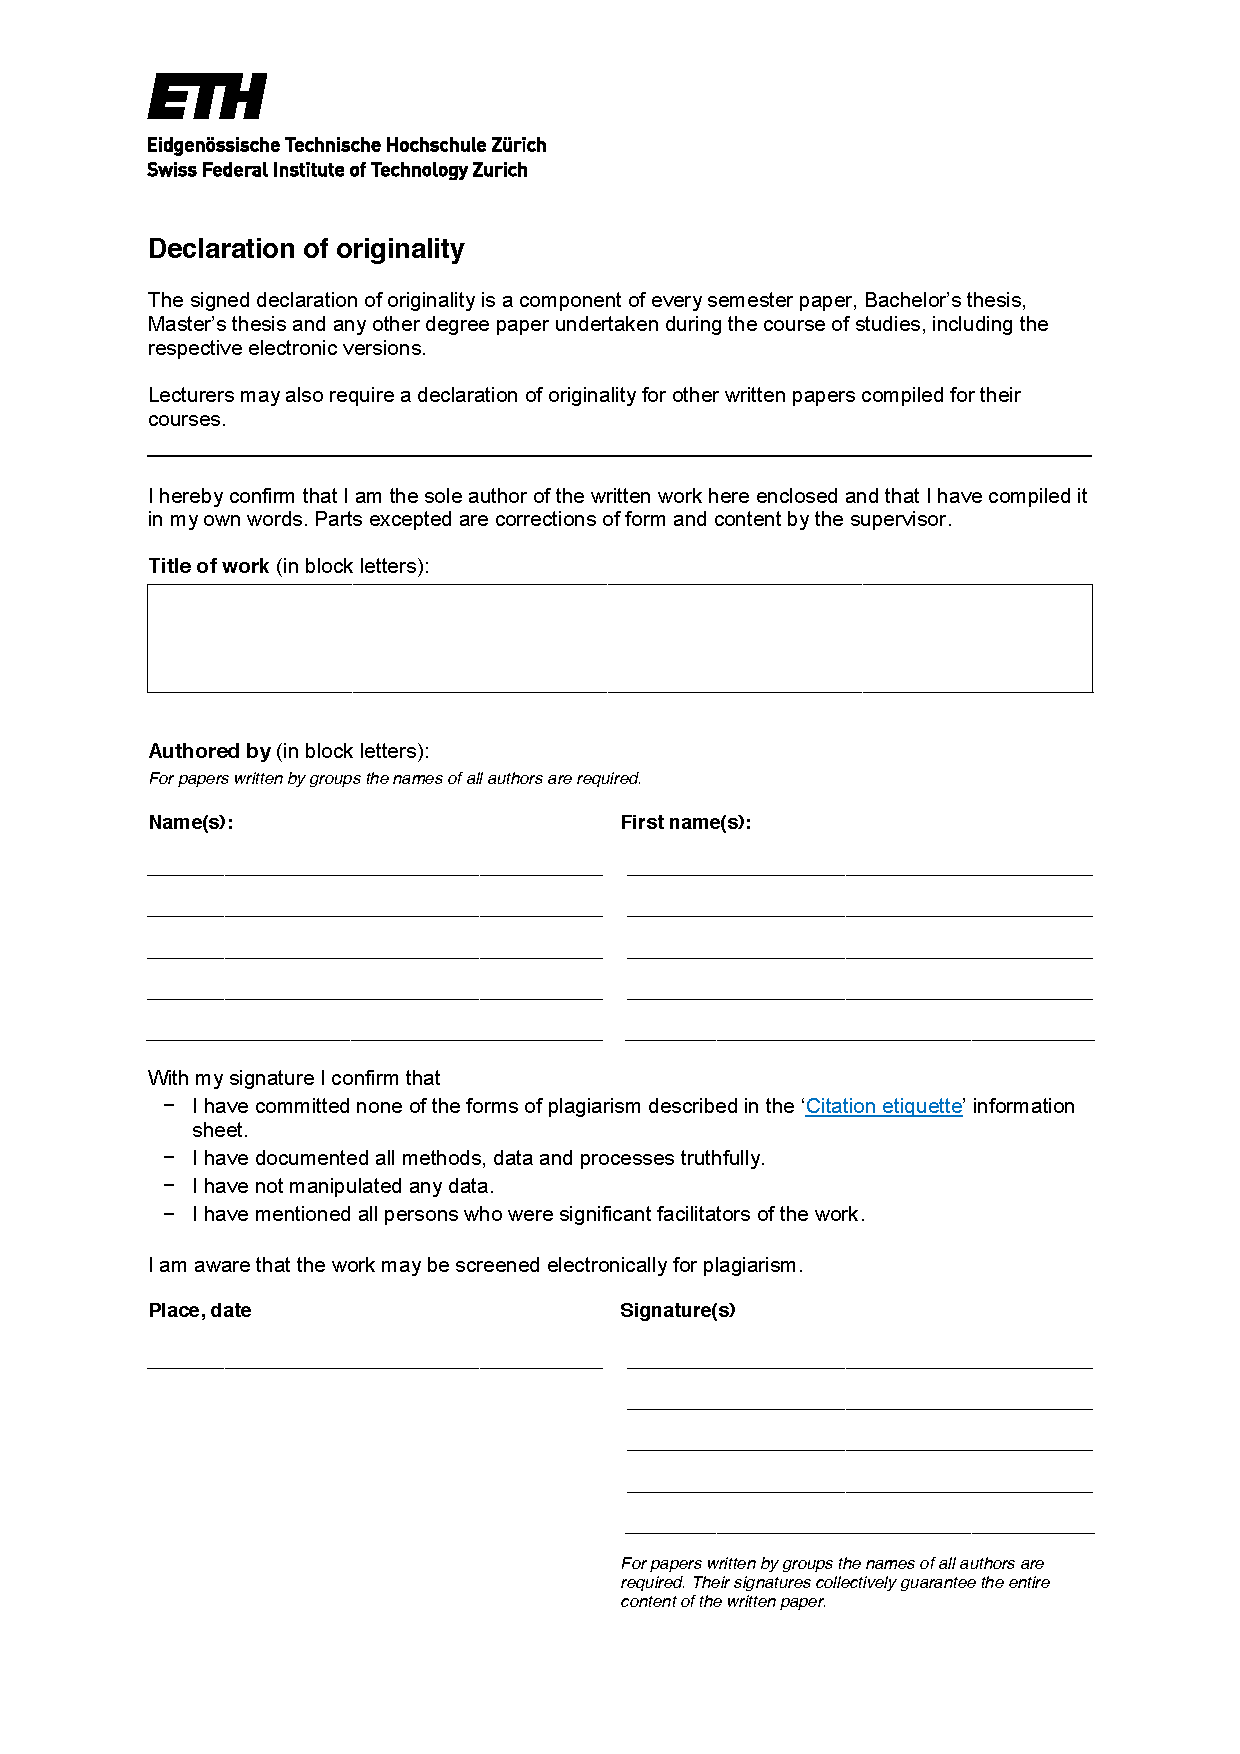
\includepdf[pages={-}]{declaration-originality.pdf}

\end{document}
